% Copyright 2004 by Till Tantau <tantau@users.sourceforge.net>.
%
% In principle, this file can be redistributed and/or modified under
% the terms of the GNU Public License, version 2.
%
% However, this file is supposed to be a template to be modified
% for your own needs. For this reason, if you use this file as a
% template and not specifically distribute it as part of a another
% package/program, I grant the extra permission to freely copy and
% modify this file as you see fit and even to delete this copyright
% notice. 

\documentclass{beamer}
\usepackage[utf8x]{inputenc}
\usepackage[T1]{fontenc}
\usepackage{lmodern}
\usepackage{subcaption}
\usepackage[slovene]{babel}
\usepackage{hyperref}
\newcommand{\vect}[1]{\boldsymbol{#1}}


\selectlanguage{slovene}
% There are many different themes available for Beamer. A comprehensive
% list with examples is given here:
% http://deic.uab.es/~iblanes/beamer_gallery/index_by_theme.html
% You can uncomment the themes below if you would like to use a different
% one:
%\usetheme{AnnArbor}
%\usetheme{Antibes}
%\usetheme{Bergen}
%\usetheme{Berkeley}
%\usetheme{Berlin}
%\usetheme{Boadilla}
%\usetheme{boxes}
%\usetheme{CambridgeUS}
%\usetheme{Copenhagen}
%\usetheme{Darmstadt}
%\usetheme{default}
%\usetheme{Frankfurt}
%\usetheme{Goettingen}
%\usetheme{Hannover}
%\usetheme{Ilmenau}
%\usetheme{JuanLesPins}
%\usetheme{Luebeck}
\usetheme{Madrid}
%\usetheme{Malmoe}
%\usetheme{Marburg}
%\usetheme{Montpellier}
%\usetheme{PaloAlto}
%\usetheme{Pittsburgh}
%\usetheme{Rochester}
%\usetheme{Singapore}
%\usetheme{Szeged}
%\usetheme{Warsaw}

\title{Sensors}

% A subtitle is optional and this may be deleted
\subtitle{Computational topology - group project}

\author[]{Nejc Kišek, Žan Klaneček}
% - Give the names in the same order as the appear in the paper.
% - Use the \inst{?} command only if the authors have different
%   affiliation.

\institute[] % (optional, but mostly needed)
{

  Faculty of computer and information science\\
  University of Ljubljana}

% - Use the \inst command only if there are several affiliations.
% - Keep it simple, no one is interested in your street address.

\date{June, 2018}
% - Either use conference name or its abbreviation.
% - Not really informative to the audience, more for people (including
%   yourself) who are reading the slides online

\subject{Computational Topology}
% This is only inserted into the PDF information catalog. Can be left
% out. 



%\AtBeginSubsection[]
%{
%  \begin{frame}<beamer>{Outline}
%    \tableofcontents[currentsection,currentsubsection]
%  \end{frame}
%+}

% Let's get started
\begin{document}

\begin{frame}
  \titlepage
\end{frame}

\begin{frame}{Outline}
  \tableofcontents
  % You might wish to add the option [pausesections]
\end{frame}

% Section and subsections will appear in the presentation overview
% and table of contents.
\section{Problem description}
\subsection{Problem}

\begin{frame}{Problem description}{}
Number of sensors on the sphere of radius 1 (Earth):
\begin{figure}[!ht]
	
	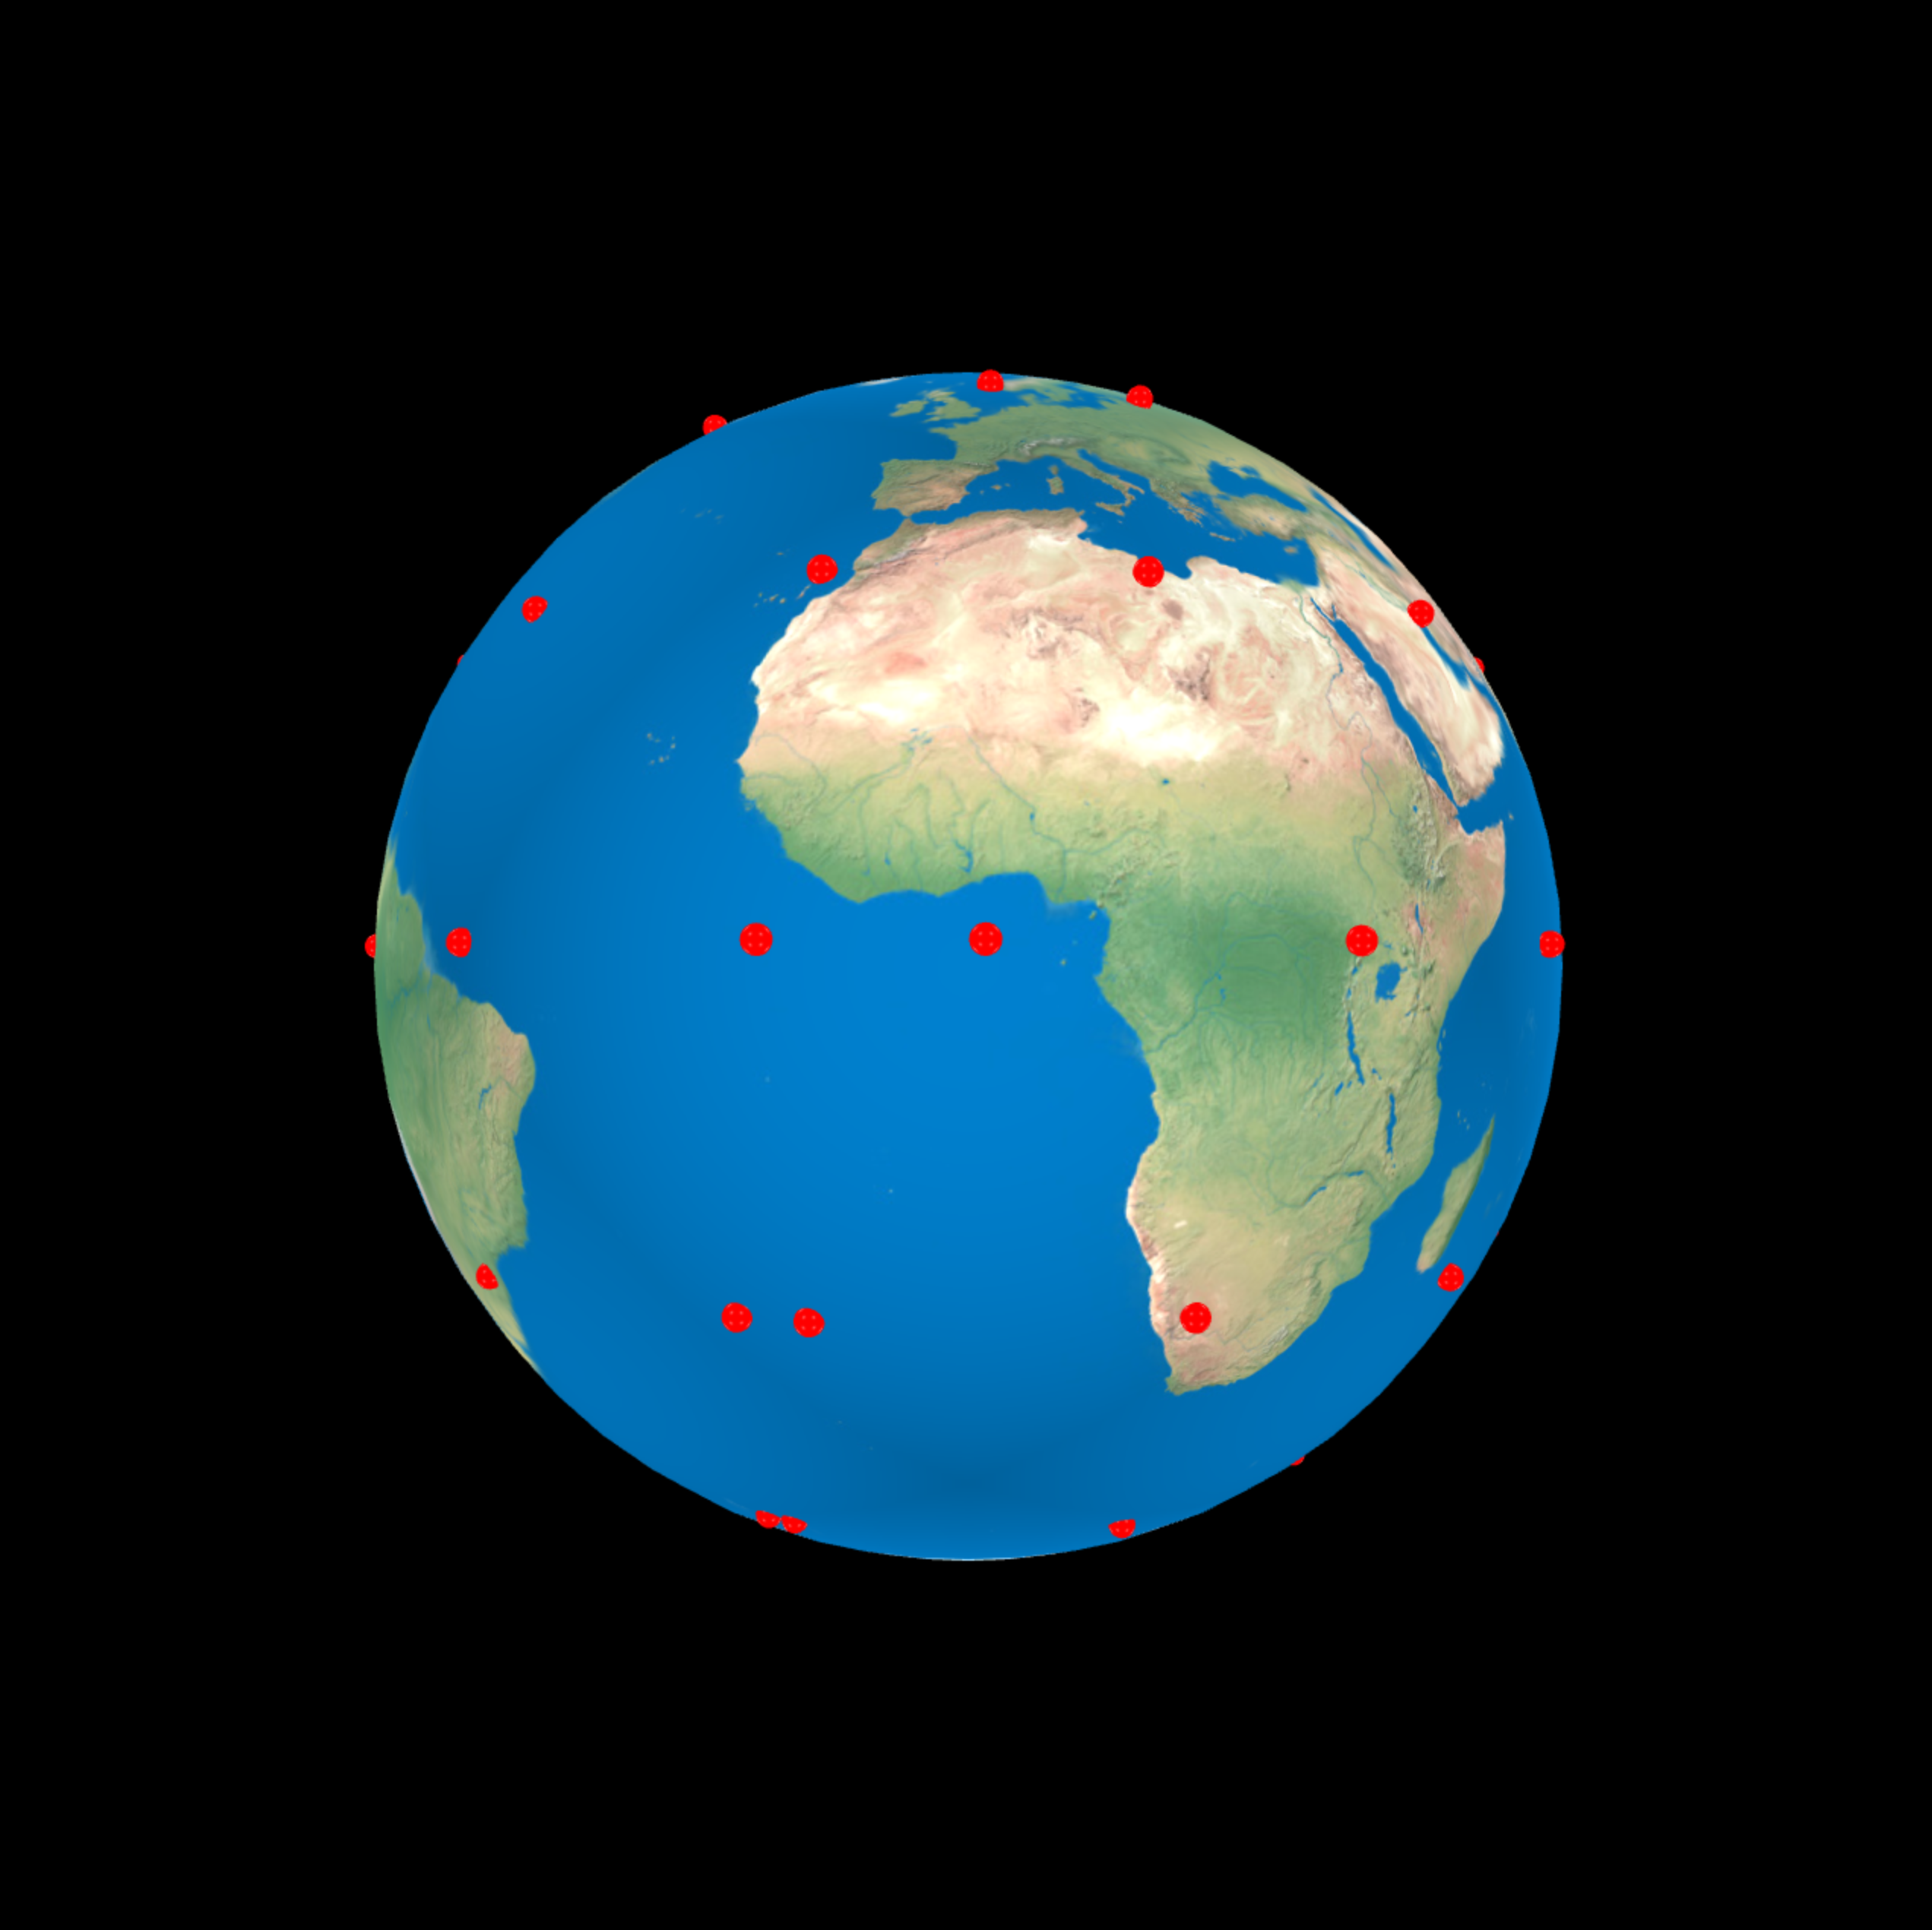
\includegraphics[scale=0.1]{used_images/sensors01}
\end{figure}
\begin{itemize}
	\item {
		each sensor gathers data from the surrounding area in the shape of a sphere of radius
		$R$,
	}
	\item {
		each sensor can communicate with other sensors which are at most $r$ away.
	}
\end{itemize}


\end{frame}
\subsection{Goals}
\begin{frame}{Goals}{}

\begin{enumerate}
	\item {The sensor network is connected.}
	\item {The sensor network covers the whole sphere.}
	\item {Values of $r$ and $R$ are as small as possible.}
	\item {There are no obsolete sensors.}
	\item {Find optimal distribution of 50 sensors on the sphere.}
\end{enumerate}

\end{frame}

\section{Topological solution}

\subsection{Vietoris-Rips complex}

\begin{frame}{Vietoris-Rips complex $\longrightarrow r$}{}
\textbf{Connected sensor network} $\longrightarrow$ Such r so that Vietoris-Rips complex $VR_r(S)$ is connected.
  \begin{itemize}
  	\item {sensors: S $\big(S_i = (r_i, \phi_i, \theta_i)\big)$,}
  	\item {sensor connections $\{S_i, S_j\} \subset S; d(S_i, S_j) \leq 2r$,}
  	\item {$F \subset S$ is a simplex in $VR_r(S)$, if diam $F \leq 2r$}.
  \end{itemize}
\end{frame}
\subsection{Čech complex}

\begin{frame}{Čech complex $\longrightarrow R$}{}
\textbf{The sensor network covers the whole sphere} $\longrightarrow$ Such R so that Euler characteristic of Čech complex should be that of a sphere.
\begin{itemize}
	\item {sensors: S $\big(S_i = (r_i, \phi_i, \theta_i)\big)$,}
	\item {$B_R(x)$ closed ball with radius $R$ around $x$,}
	\item {$Č_R = \{\sigma \subset S,\cap_{x\in \sigma}B_R(x) \neq \emptyset \}$.\\~\
	}
\end{itemize}

In practice, instead of calculating Euler characteristic we checked first two Betti numbers.\\~\

\end{frame}

\section{Results and implementation}
\subsection{Two different initial distributions of sensors on Earth}
\begin{frame}{Two different initial distributions of sensors on Earth}

\begin{figure}[!ht]
	\centering
	\begin{subfigure}{.5\textwidth}
		\centering
		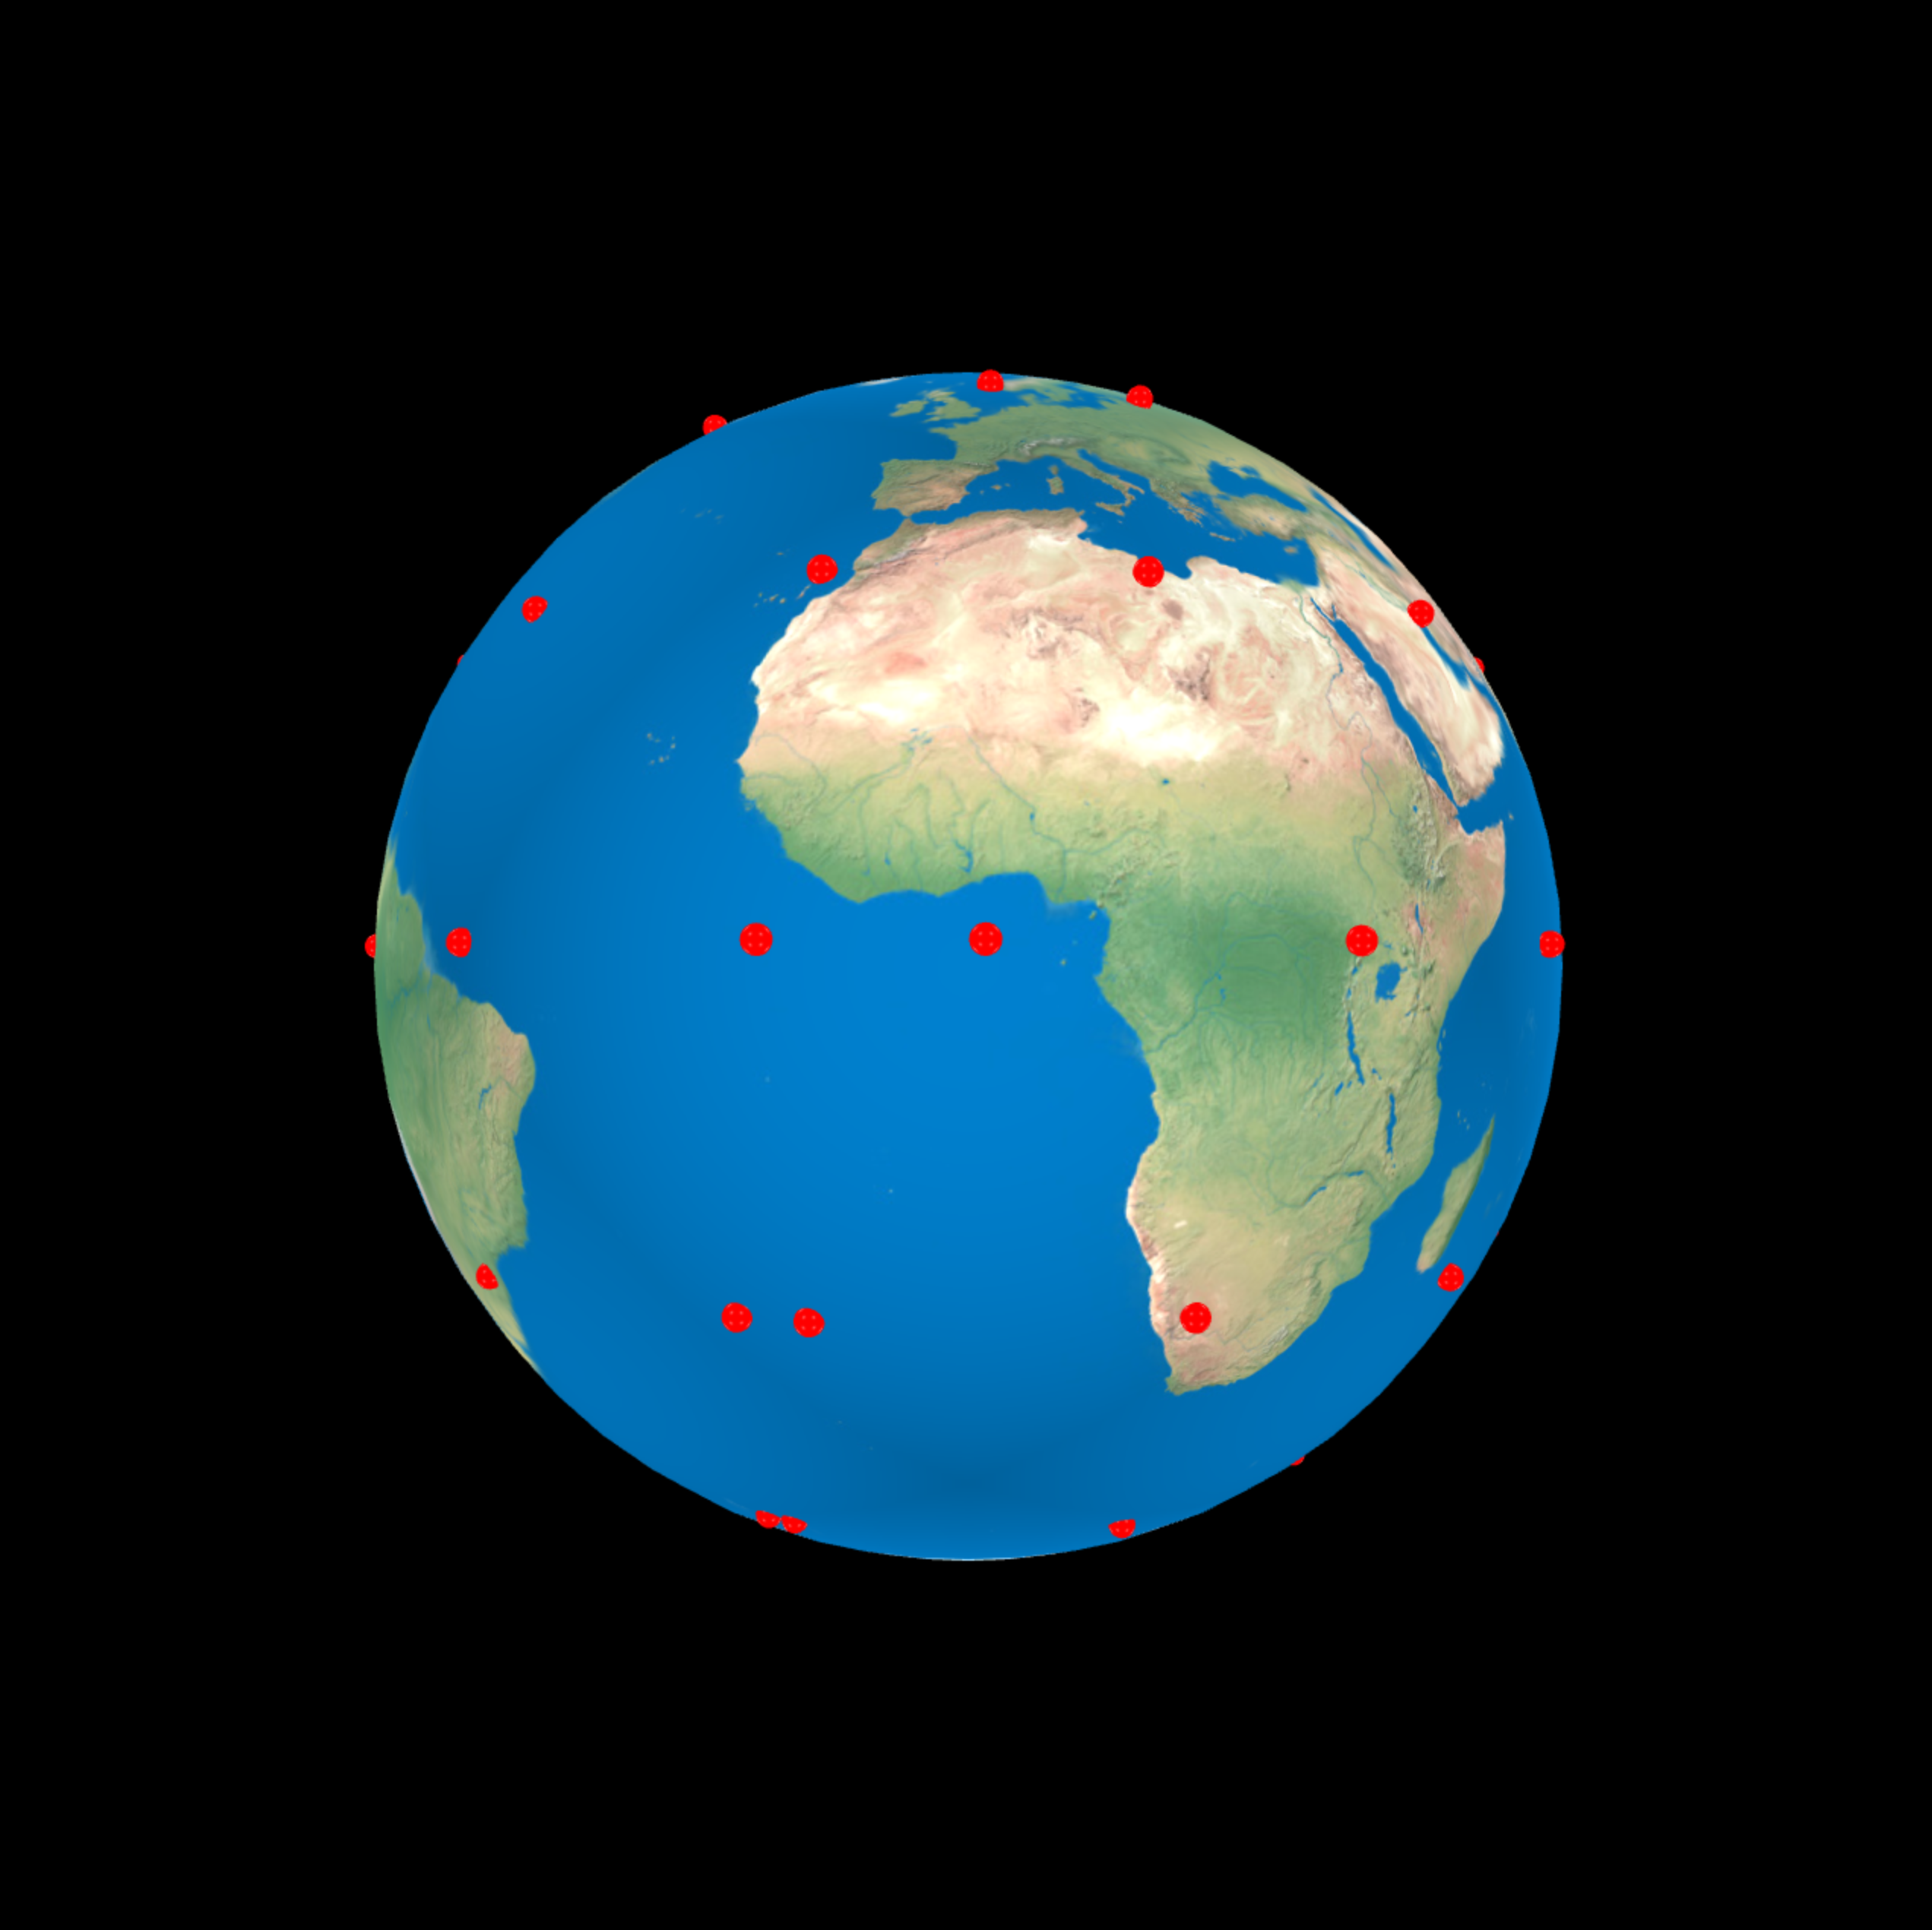
\includegraphics[scale=0.15]{used_images/sensors01.png}
		\caption{Sensors 1.}
	\end{subfigure}%
	\begin{subfigure}{.5\textwidth}
		\centering
		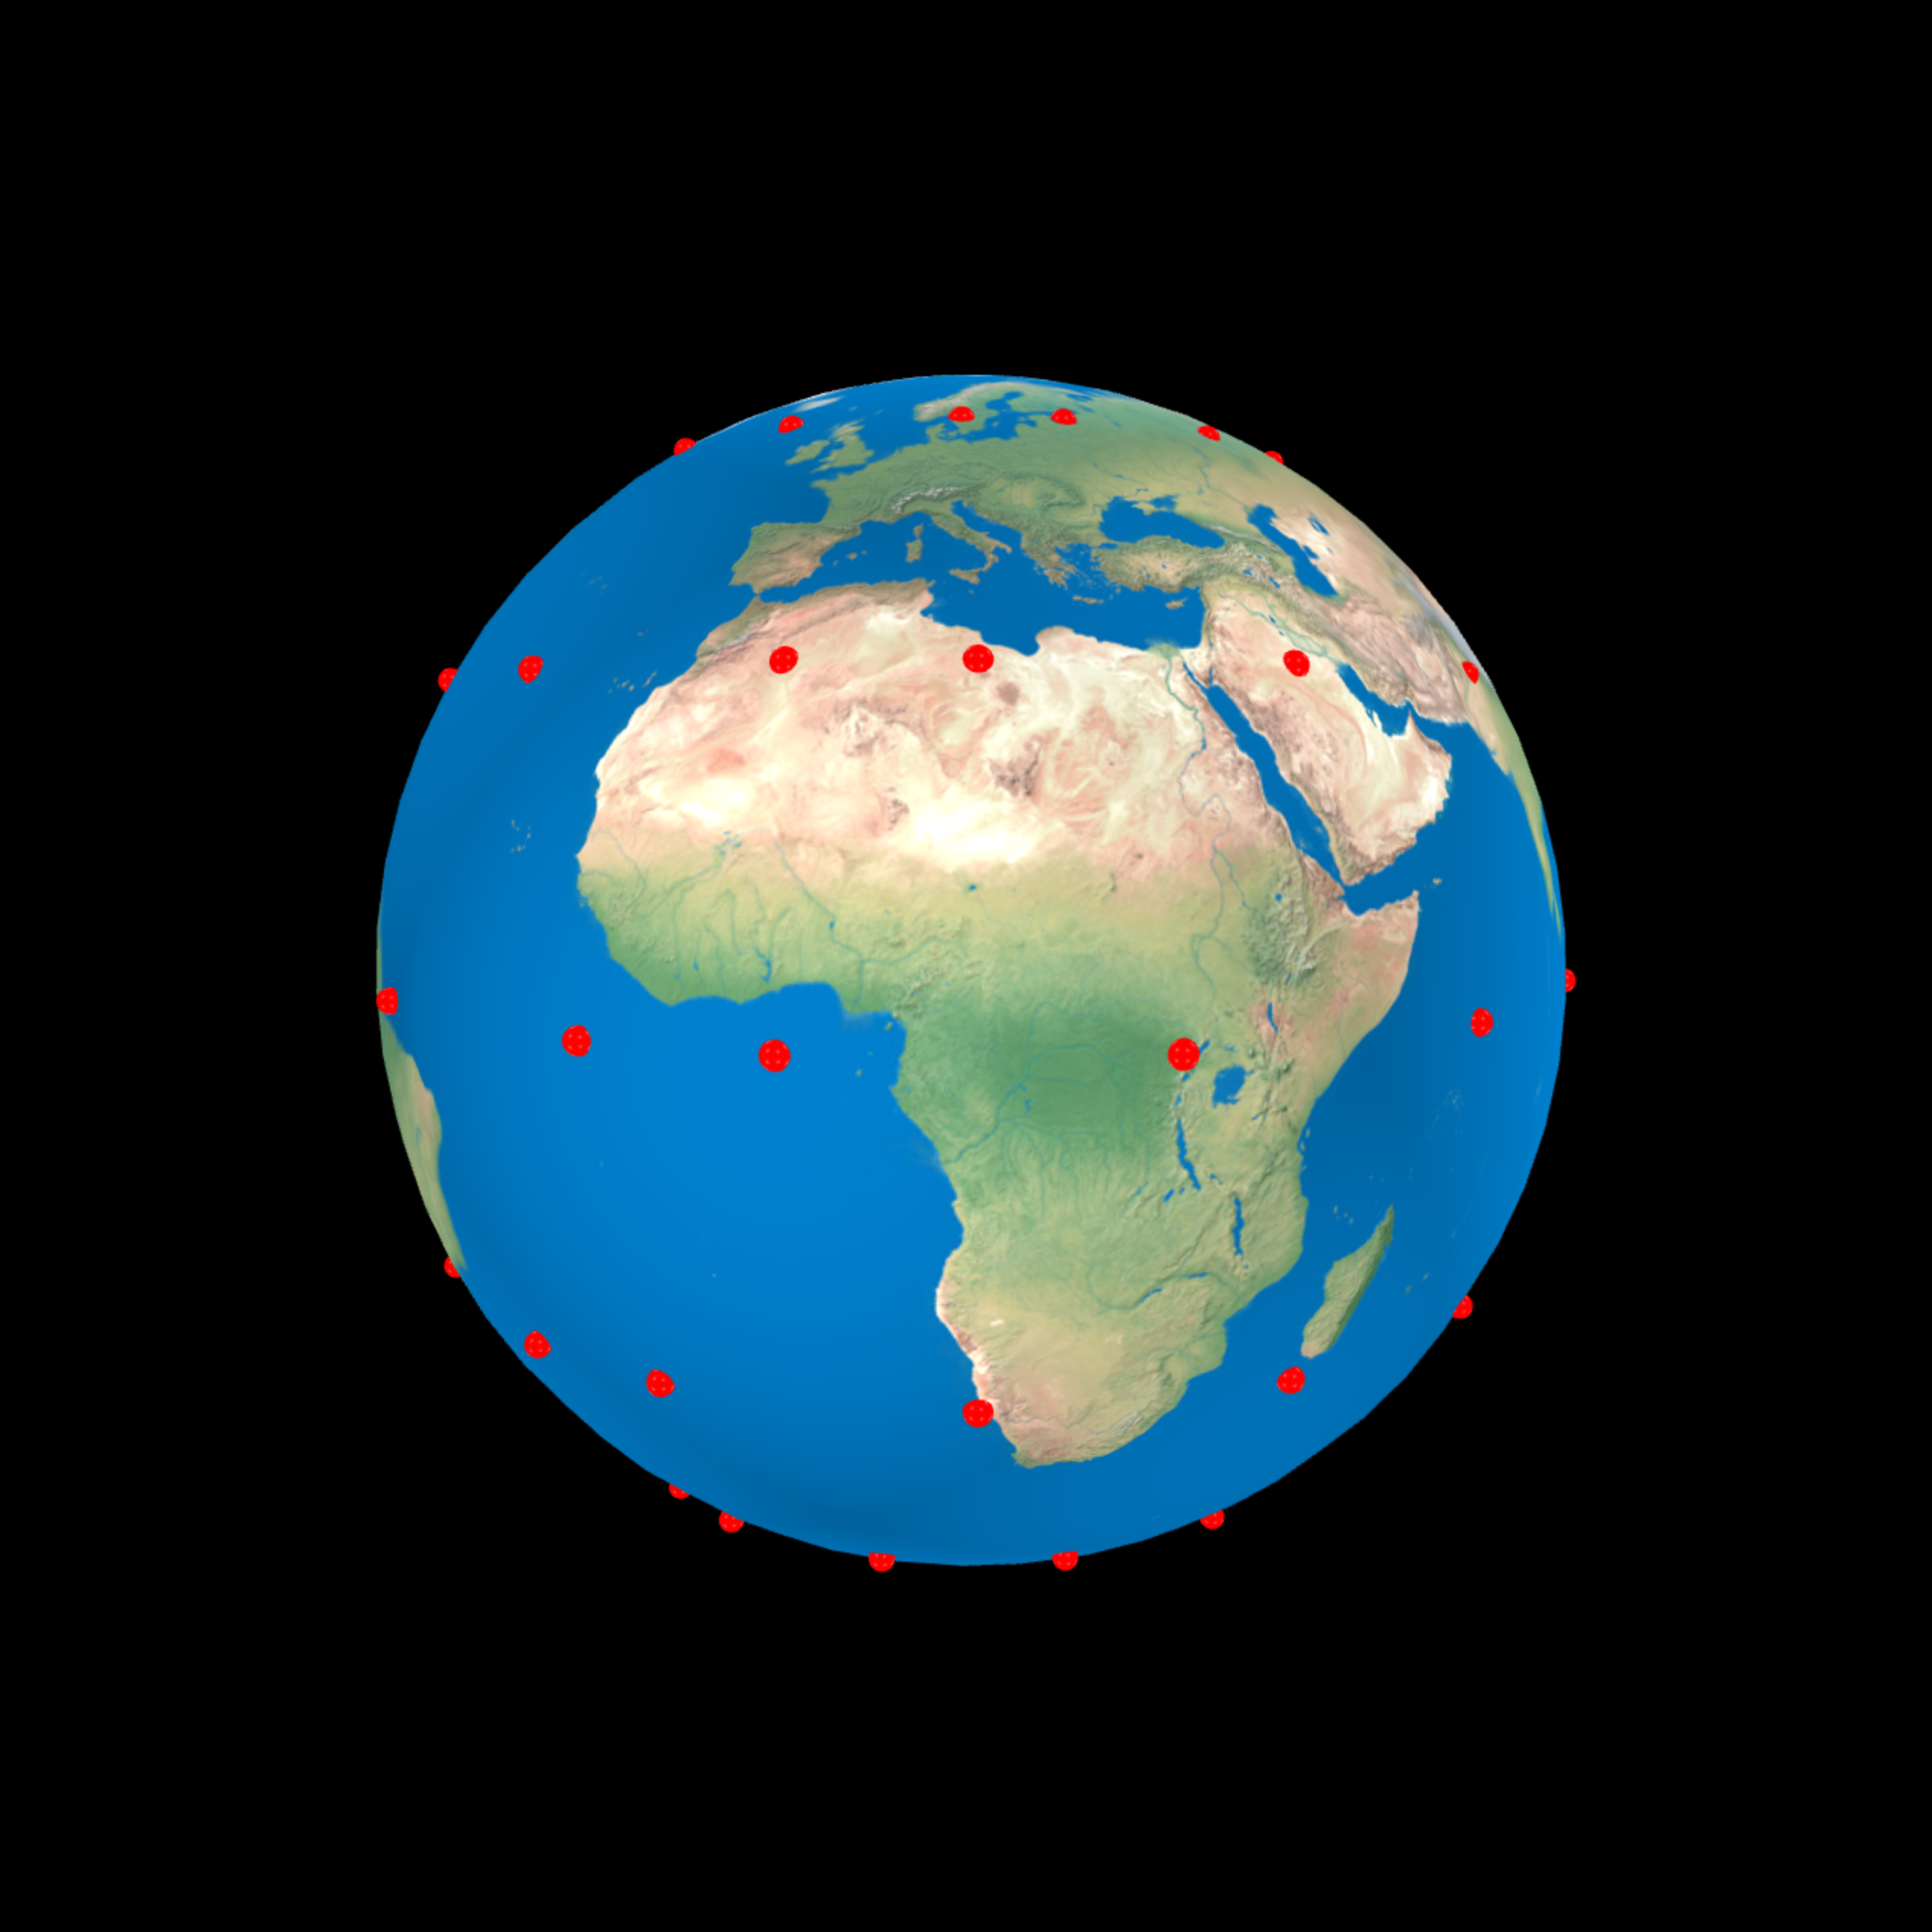
\includegraphics[scale=0.1502]{used_images/sensors02.png}
		\caption{Sensors 2.}
	\end{subfigure}%
	
\end{figure}
\end{frame}

\subsection{Vietoris-Rips $\longrightarrow$ 1 component}

\begin{frame}{Vietoris-Rips $\longrightarrow$ 1 component}
Sensor network must be connected.
\begin{figure}[!ht]
	\centering
	\begin{subfigure}{.5\textwidth}
		\centering
		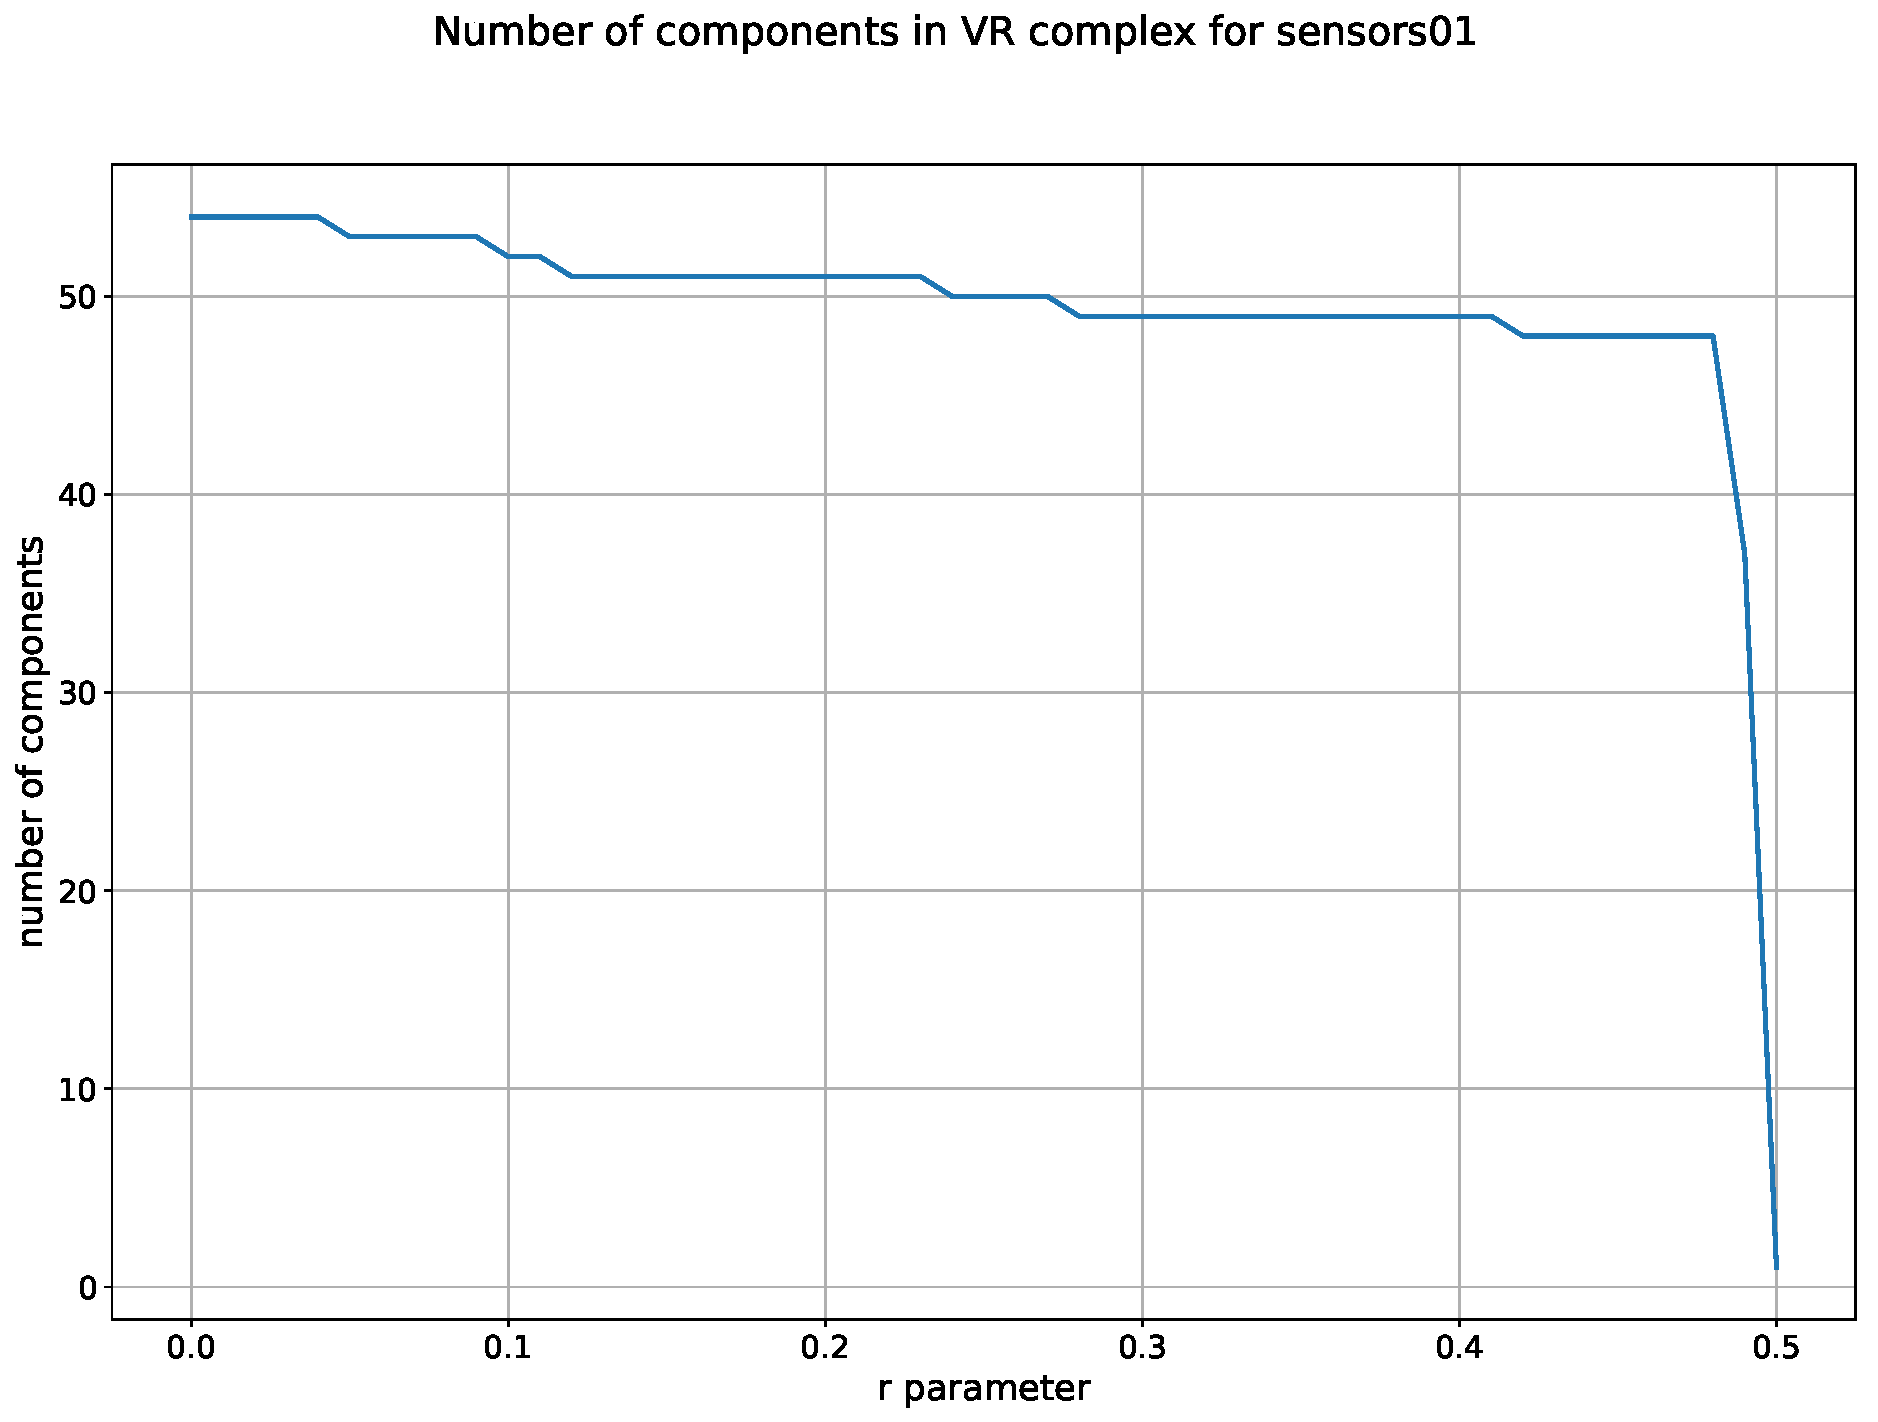
\includegraphics[scale=0.19]{used_images/plot_vr_sensors01.pdf}
		\caption{$r = 0.5$}
	\end{subfigure}%
	\begin{subfigure}{.5\textwidth}
		\centering
		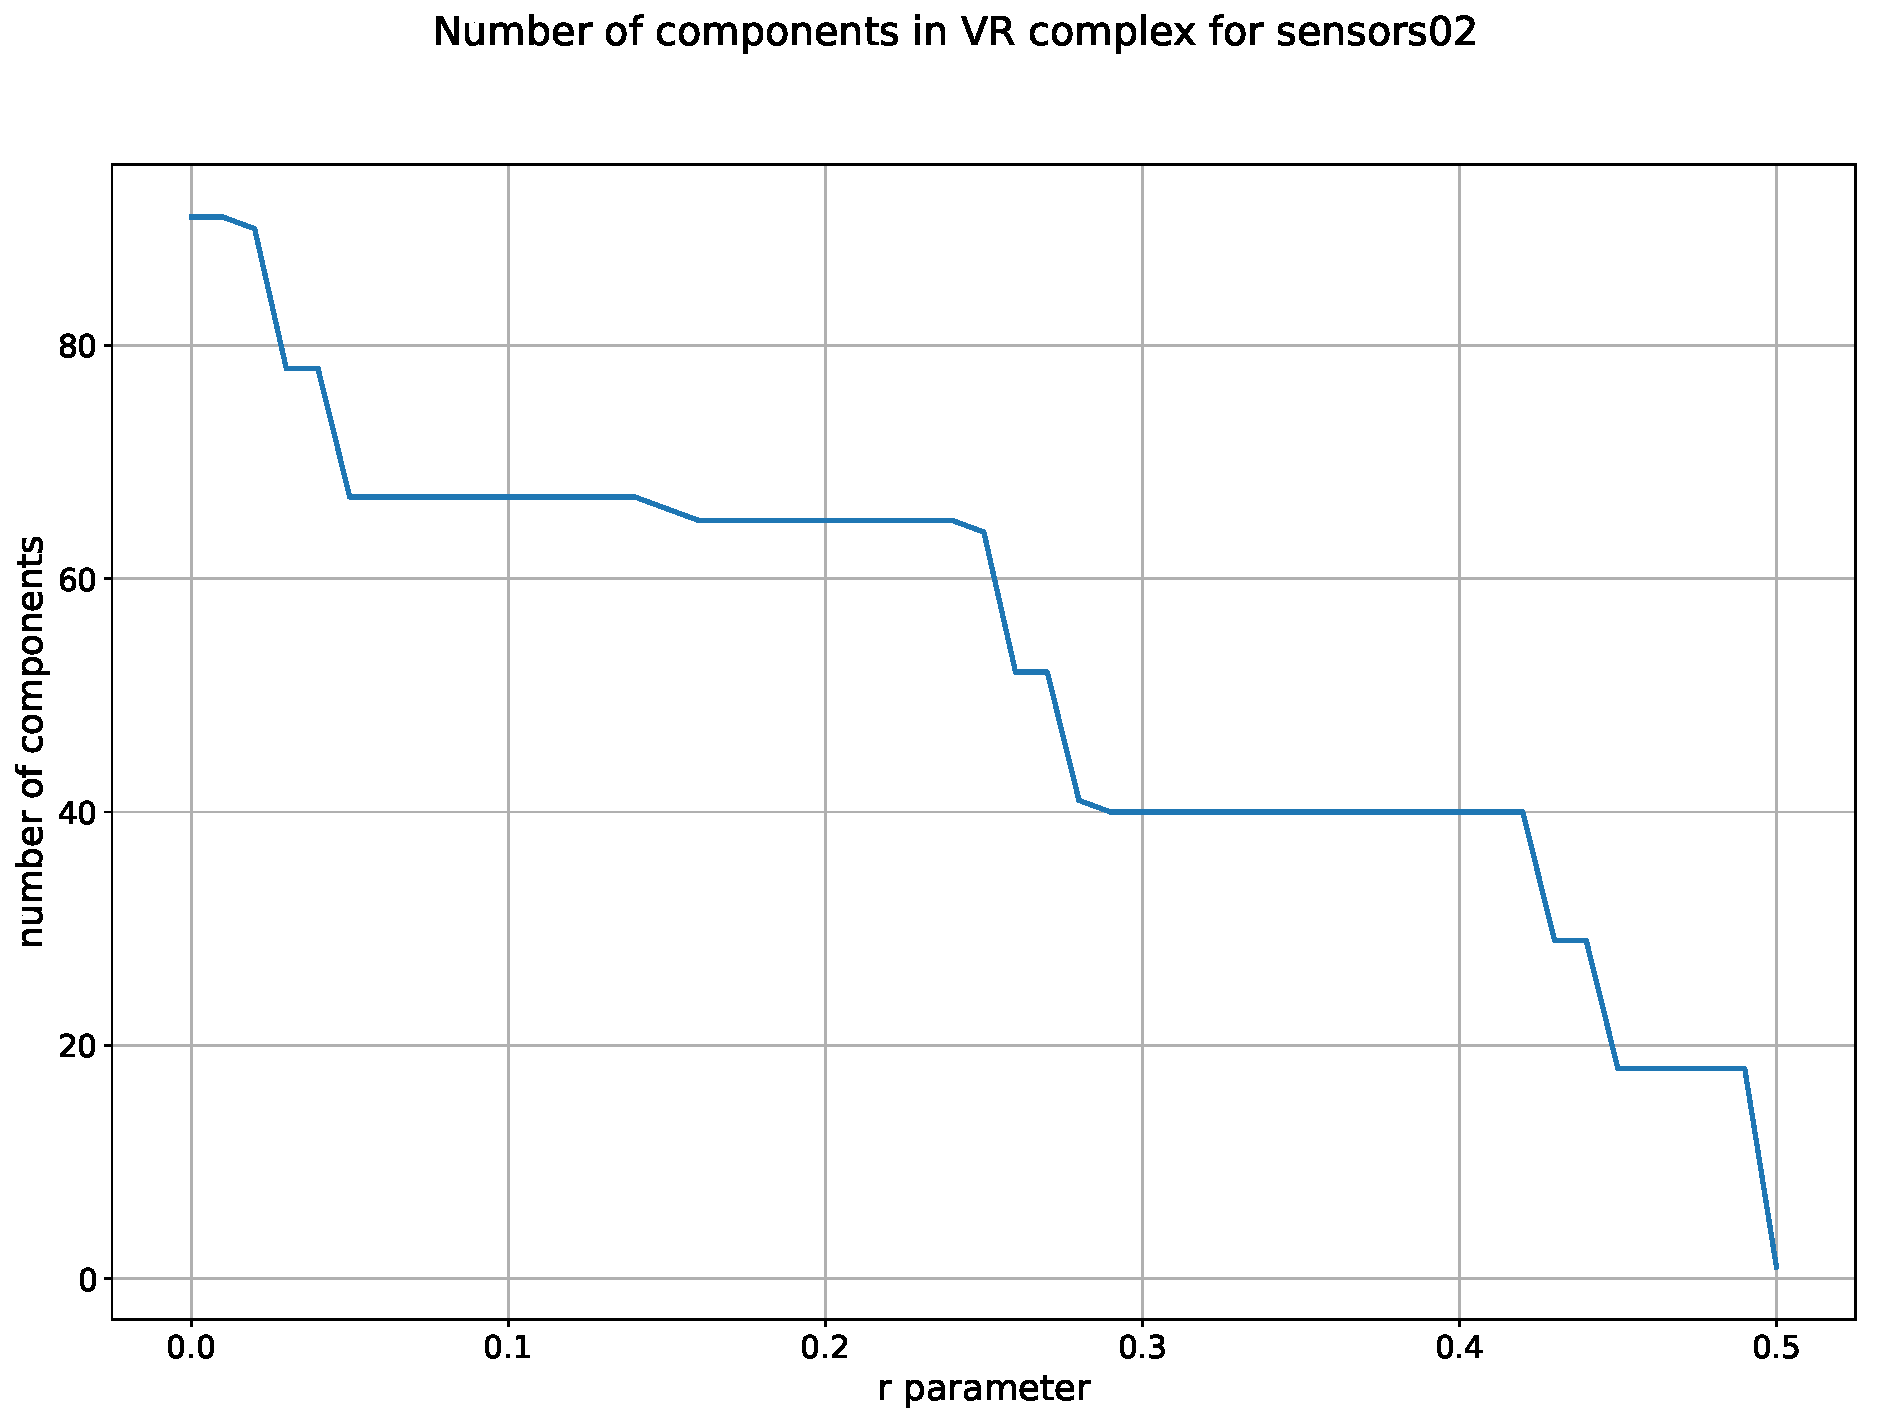
\includegraphics[scale=0.19]{used_images/plot_vr_sensors02.pdf}
		\caption{$r = 0.5$}
	\end{subfigure}%
	
\end{figure}
\end{frame}

\subsection{Barcode for Vietoris-Rips}

\begin{frame}{Barcode for Vietoris-Rips}

\begin{figure}[!ht]
	\centering
	\begin{subfigure}{.5\textwidth}
		\centering
		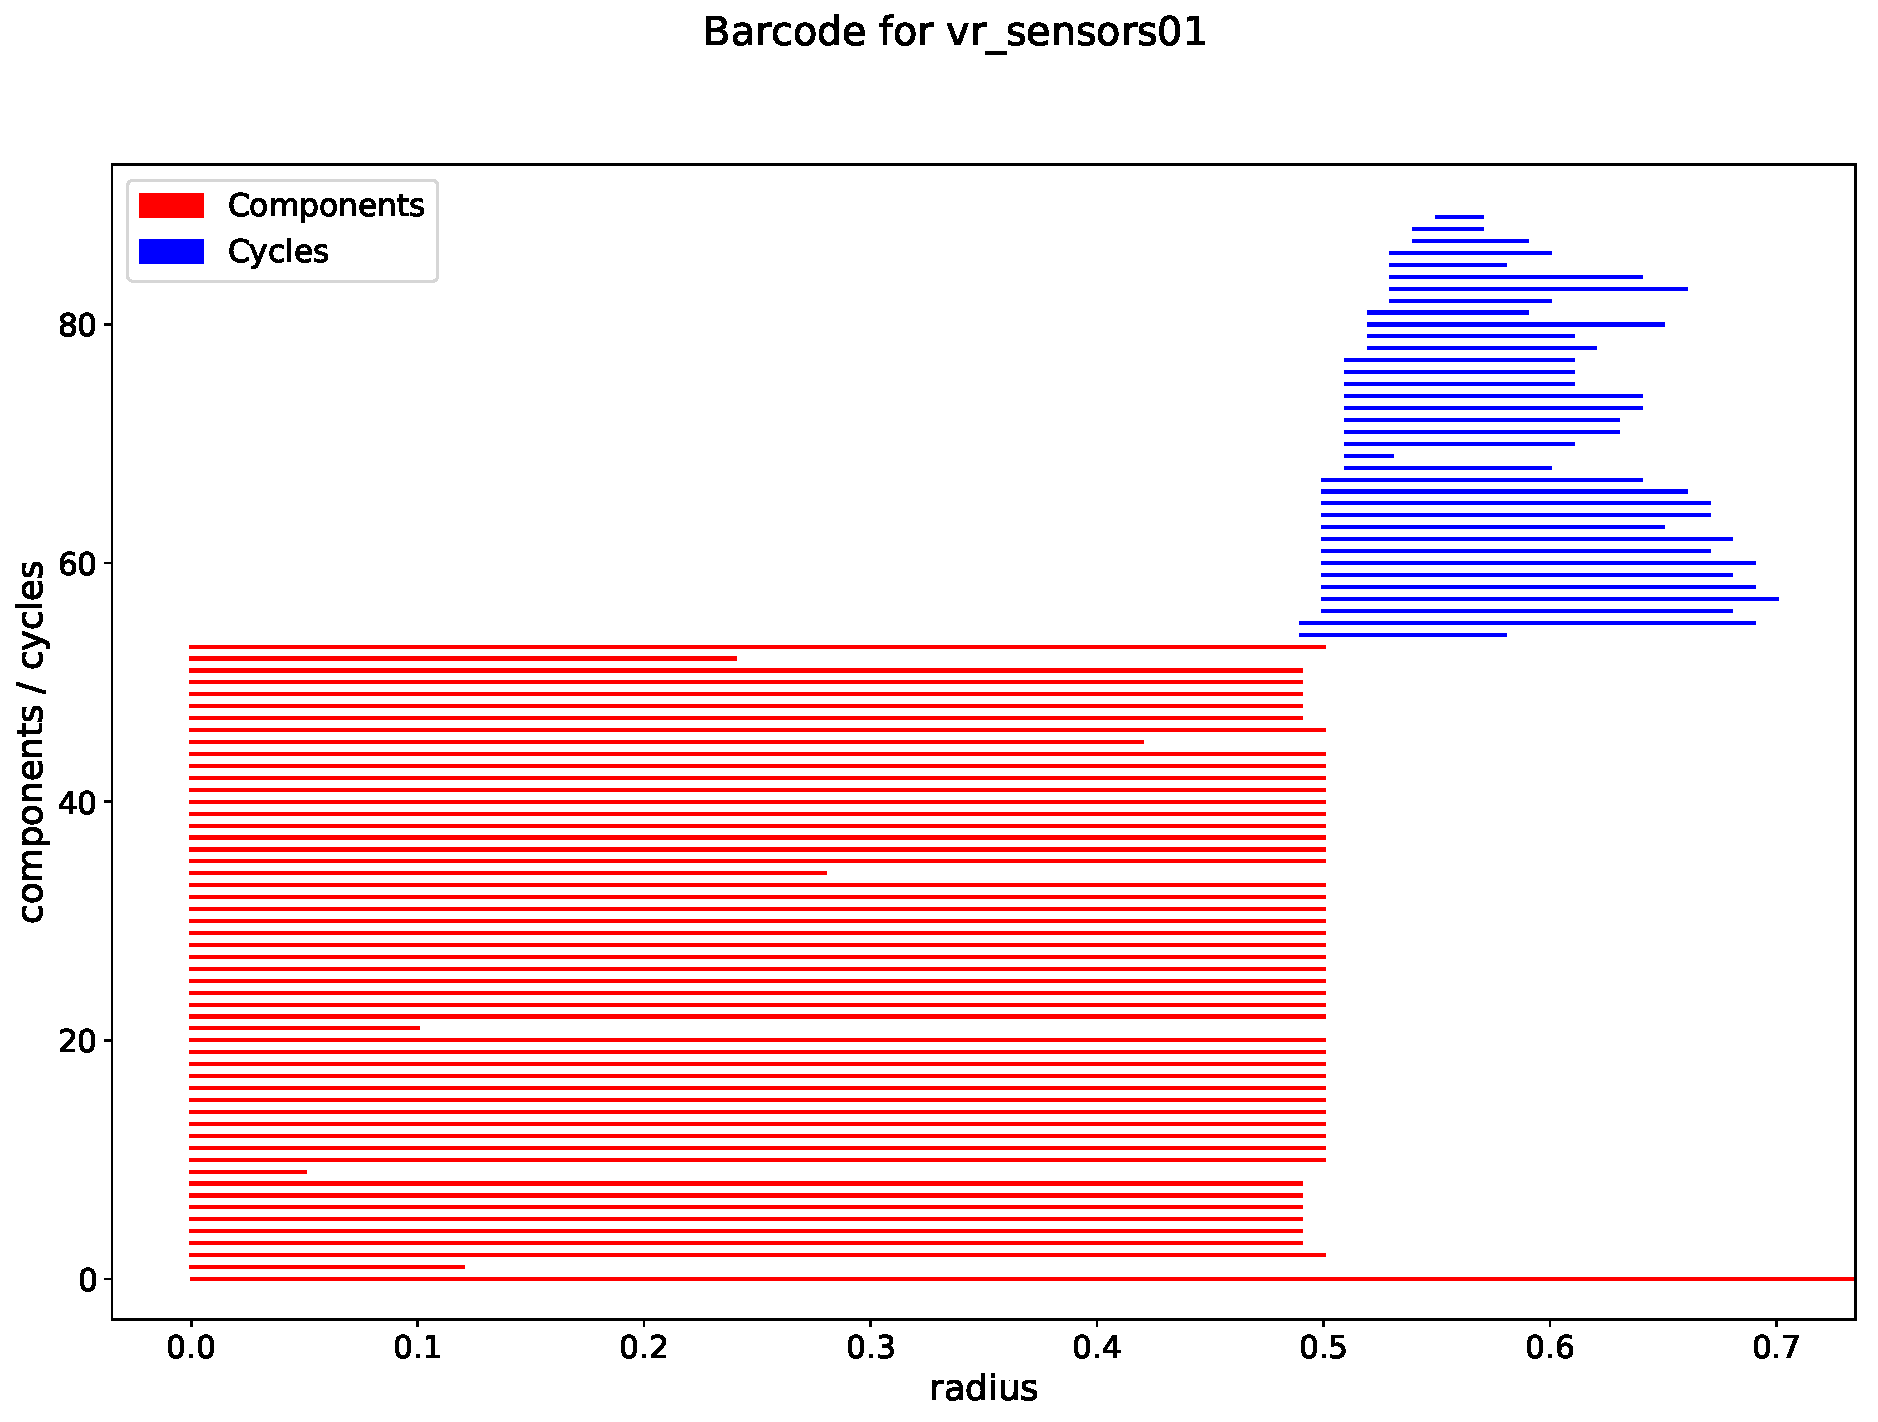
\includegraphics[scale=0.19]{used_images/barcode_vr_sensors01.pdf}
		\caption{Sensors 1.}
	\end{subfigure}%
	\begin{subfigure}{.5\textwidth}
		\centering
		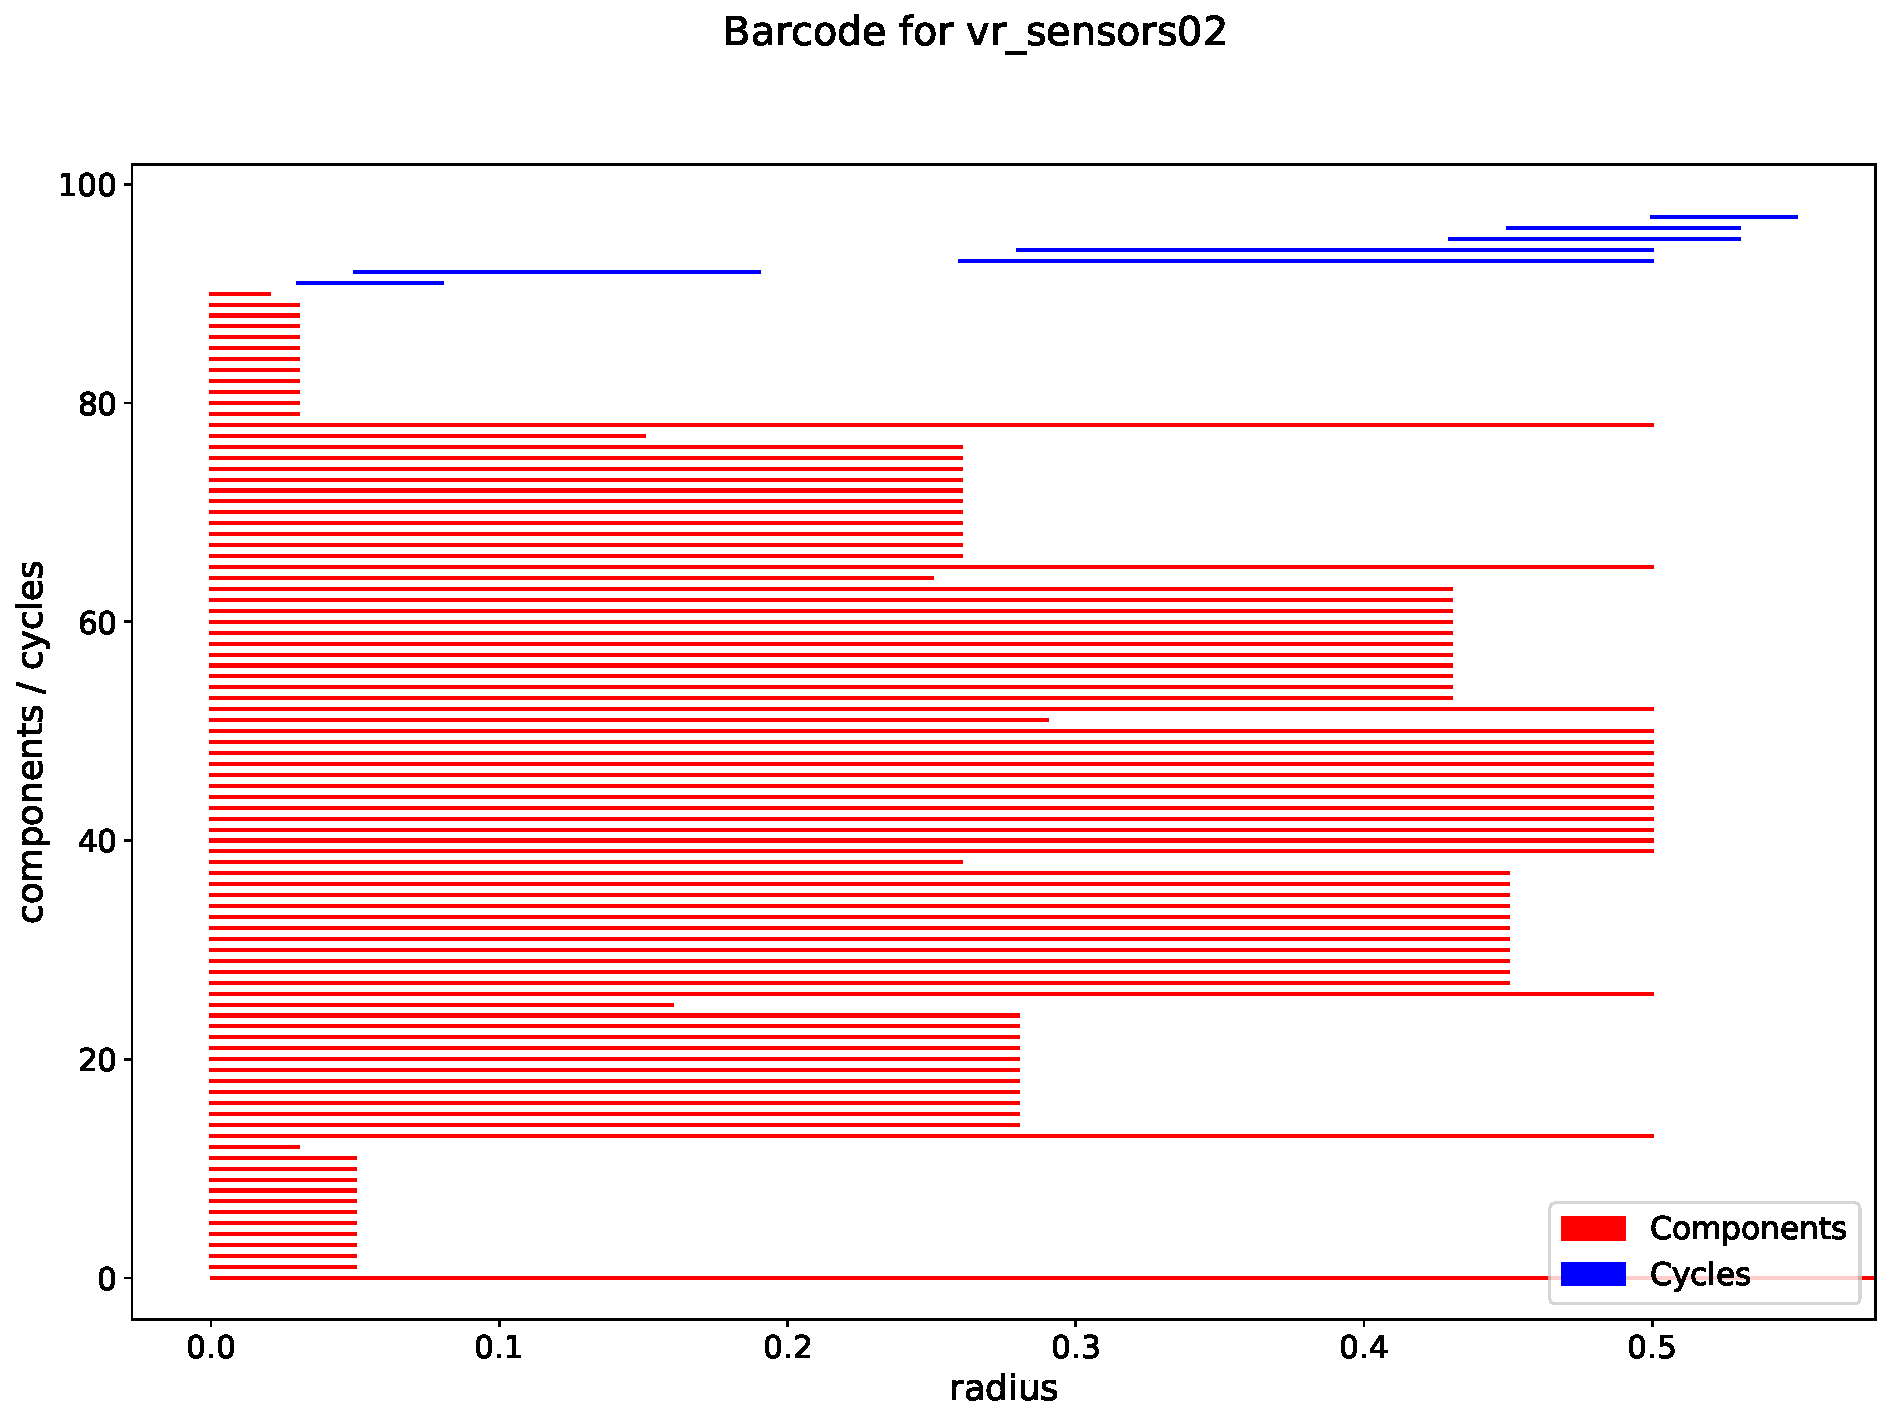
\includegraphics[scale=0.19]{used_images/barcode_vr_sensors02.pdf}
		\caption{Sensors 2.}
	\end{subfigure}%
	
\end{figure}
\end{frame}
\subsection{Connections in sensor network}
\begin{frame}{Connections in sensor network}
Drawn connections for appropriate parameter $r$.
\begin{figure}[!ht]
	\centering
	\begin{subfigure}{.5\textwidth}
		\centering
		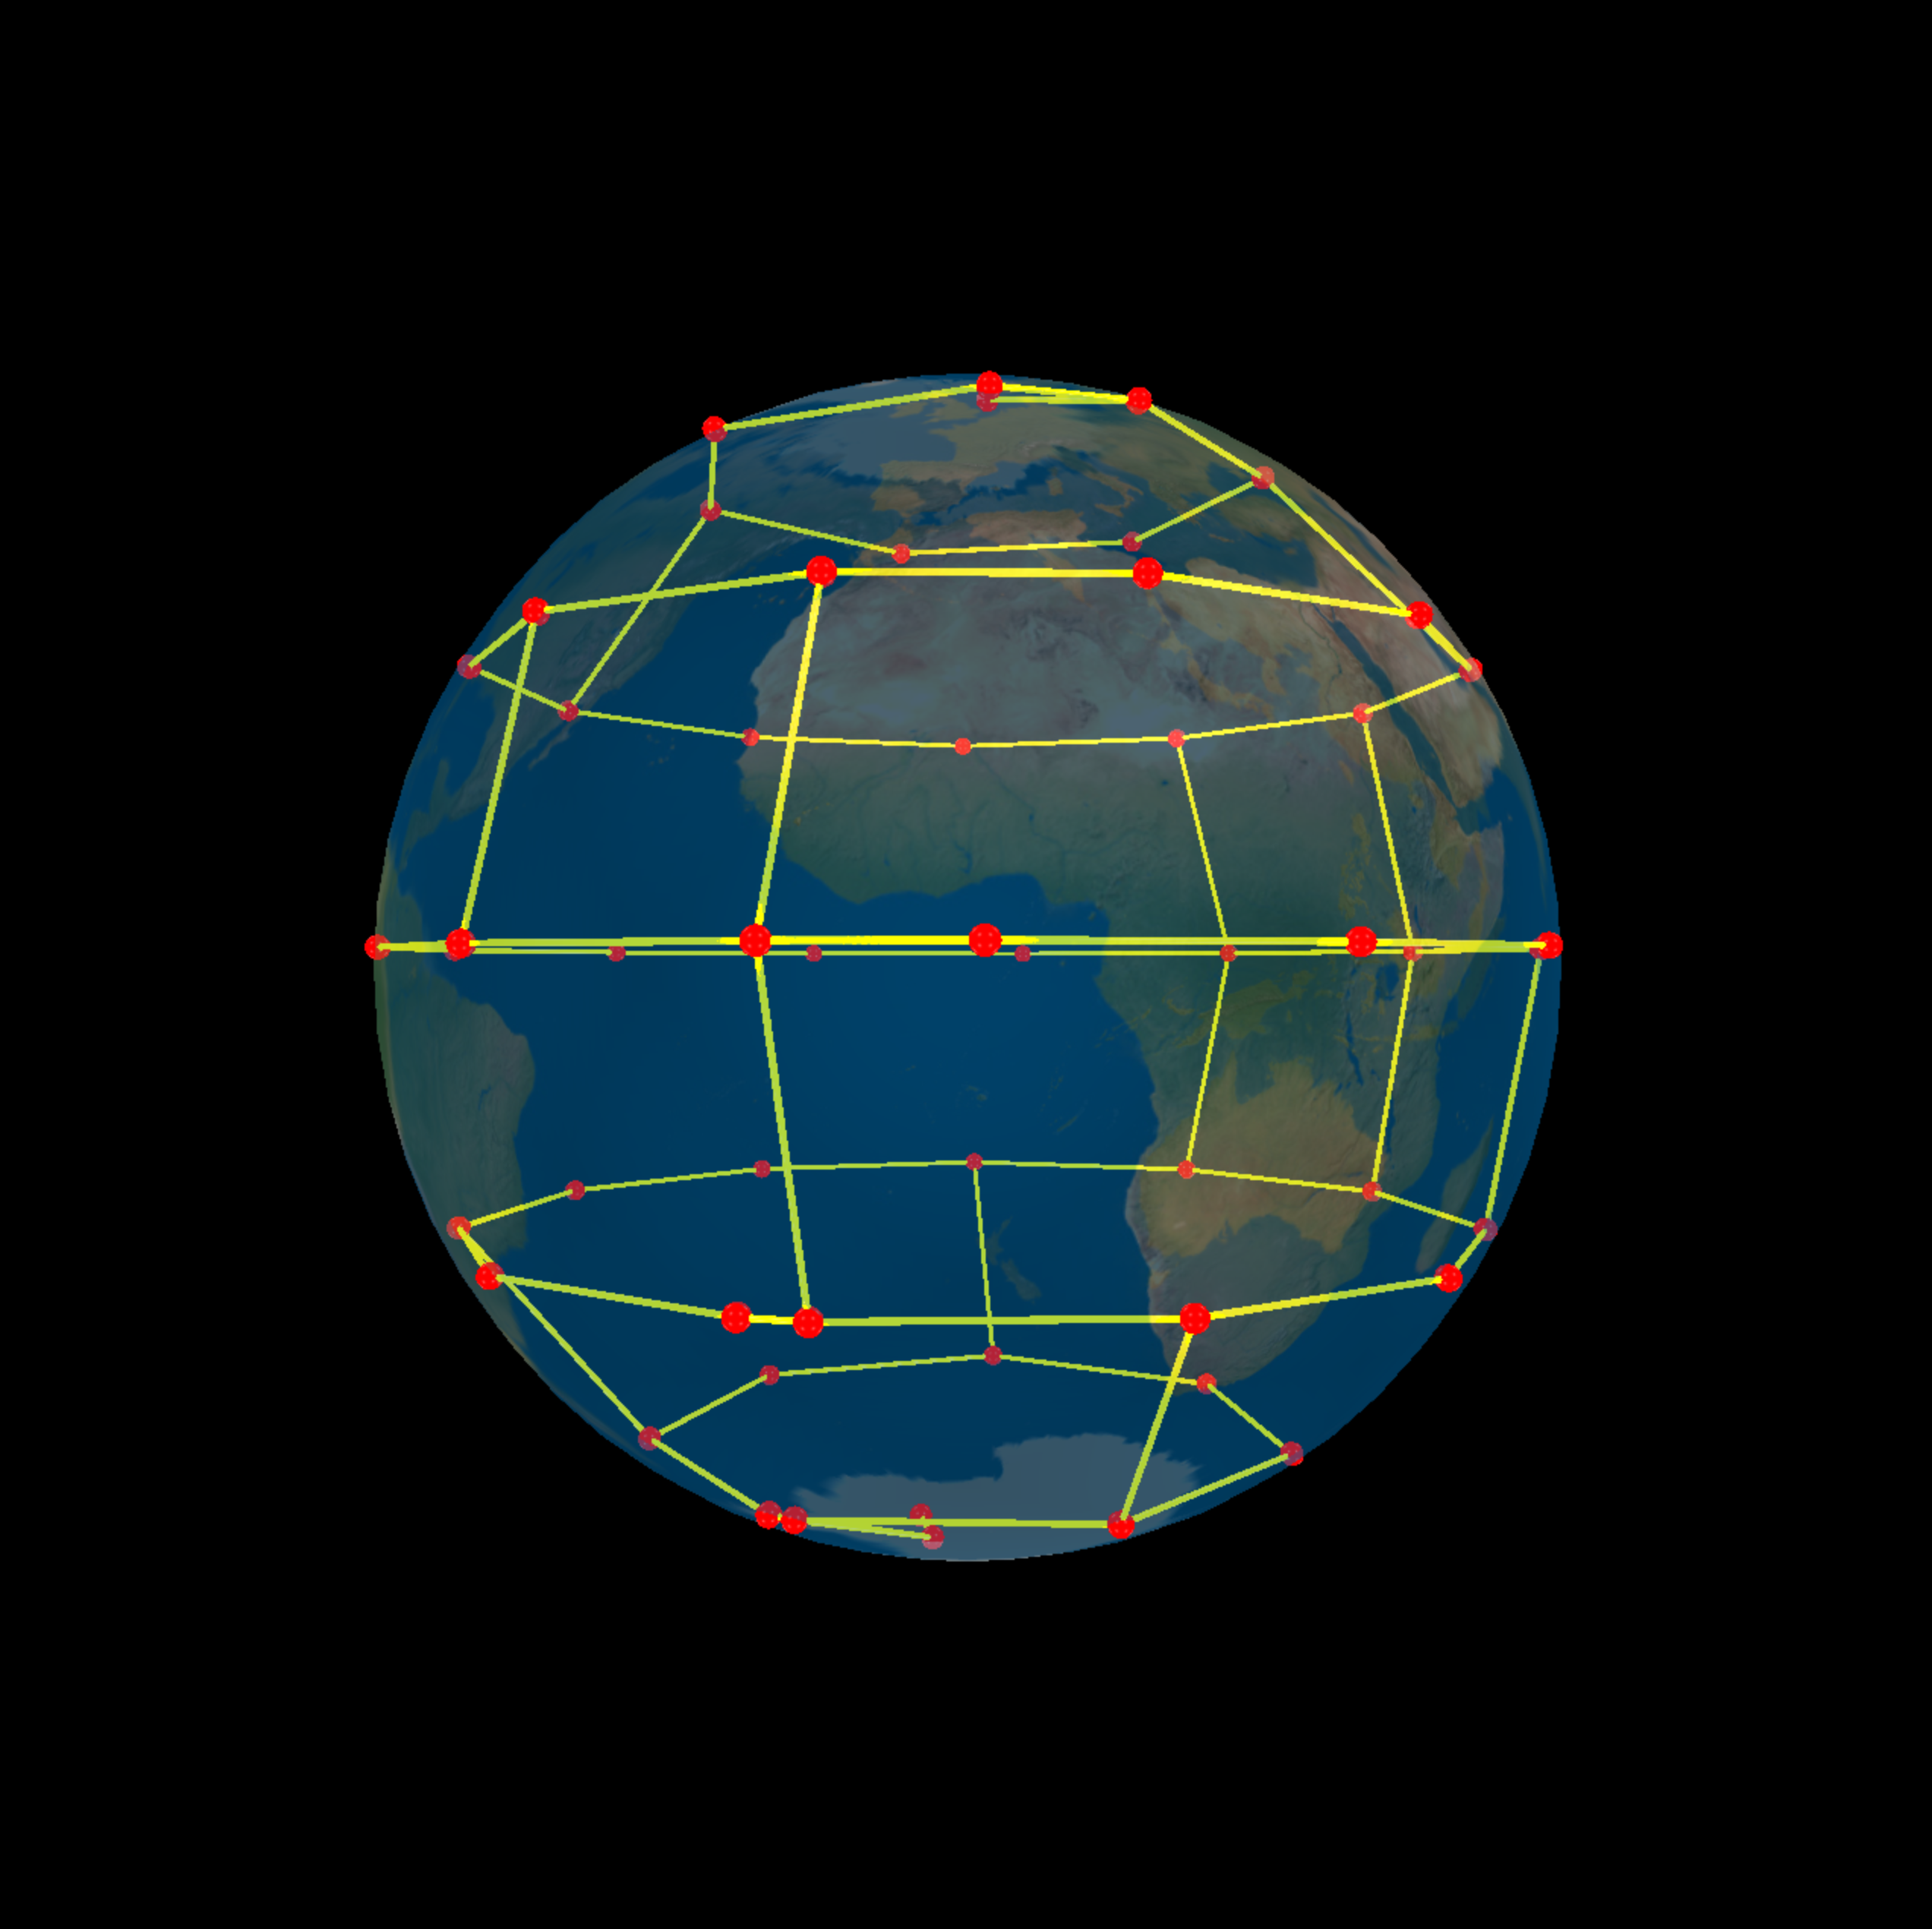
\includegraphics[scale=0.15]{used_images/connections01}
		\caption{Sensors 1: $r = 0.5$}
	\end{subfigure}%
	\begin{subfigure}{.5\textwidth}
		\centering
		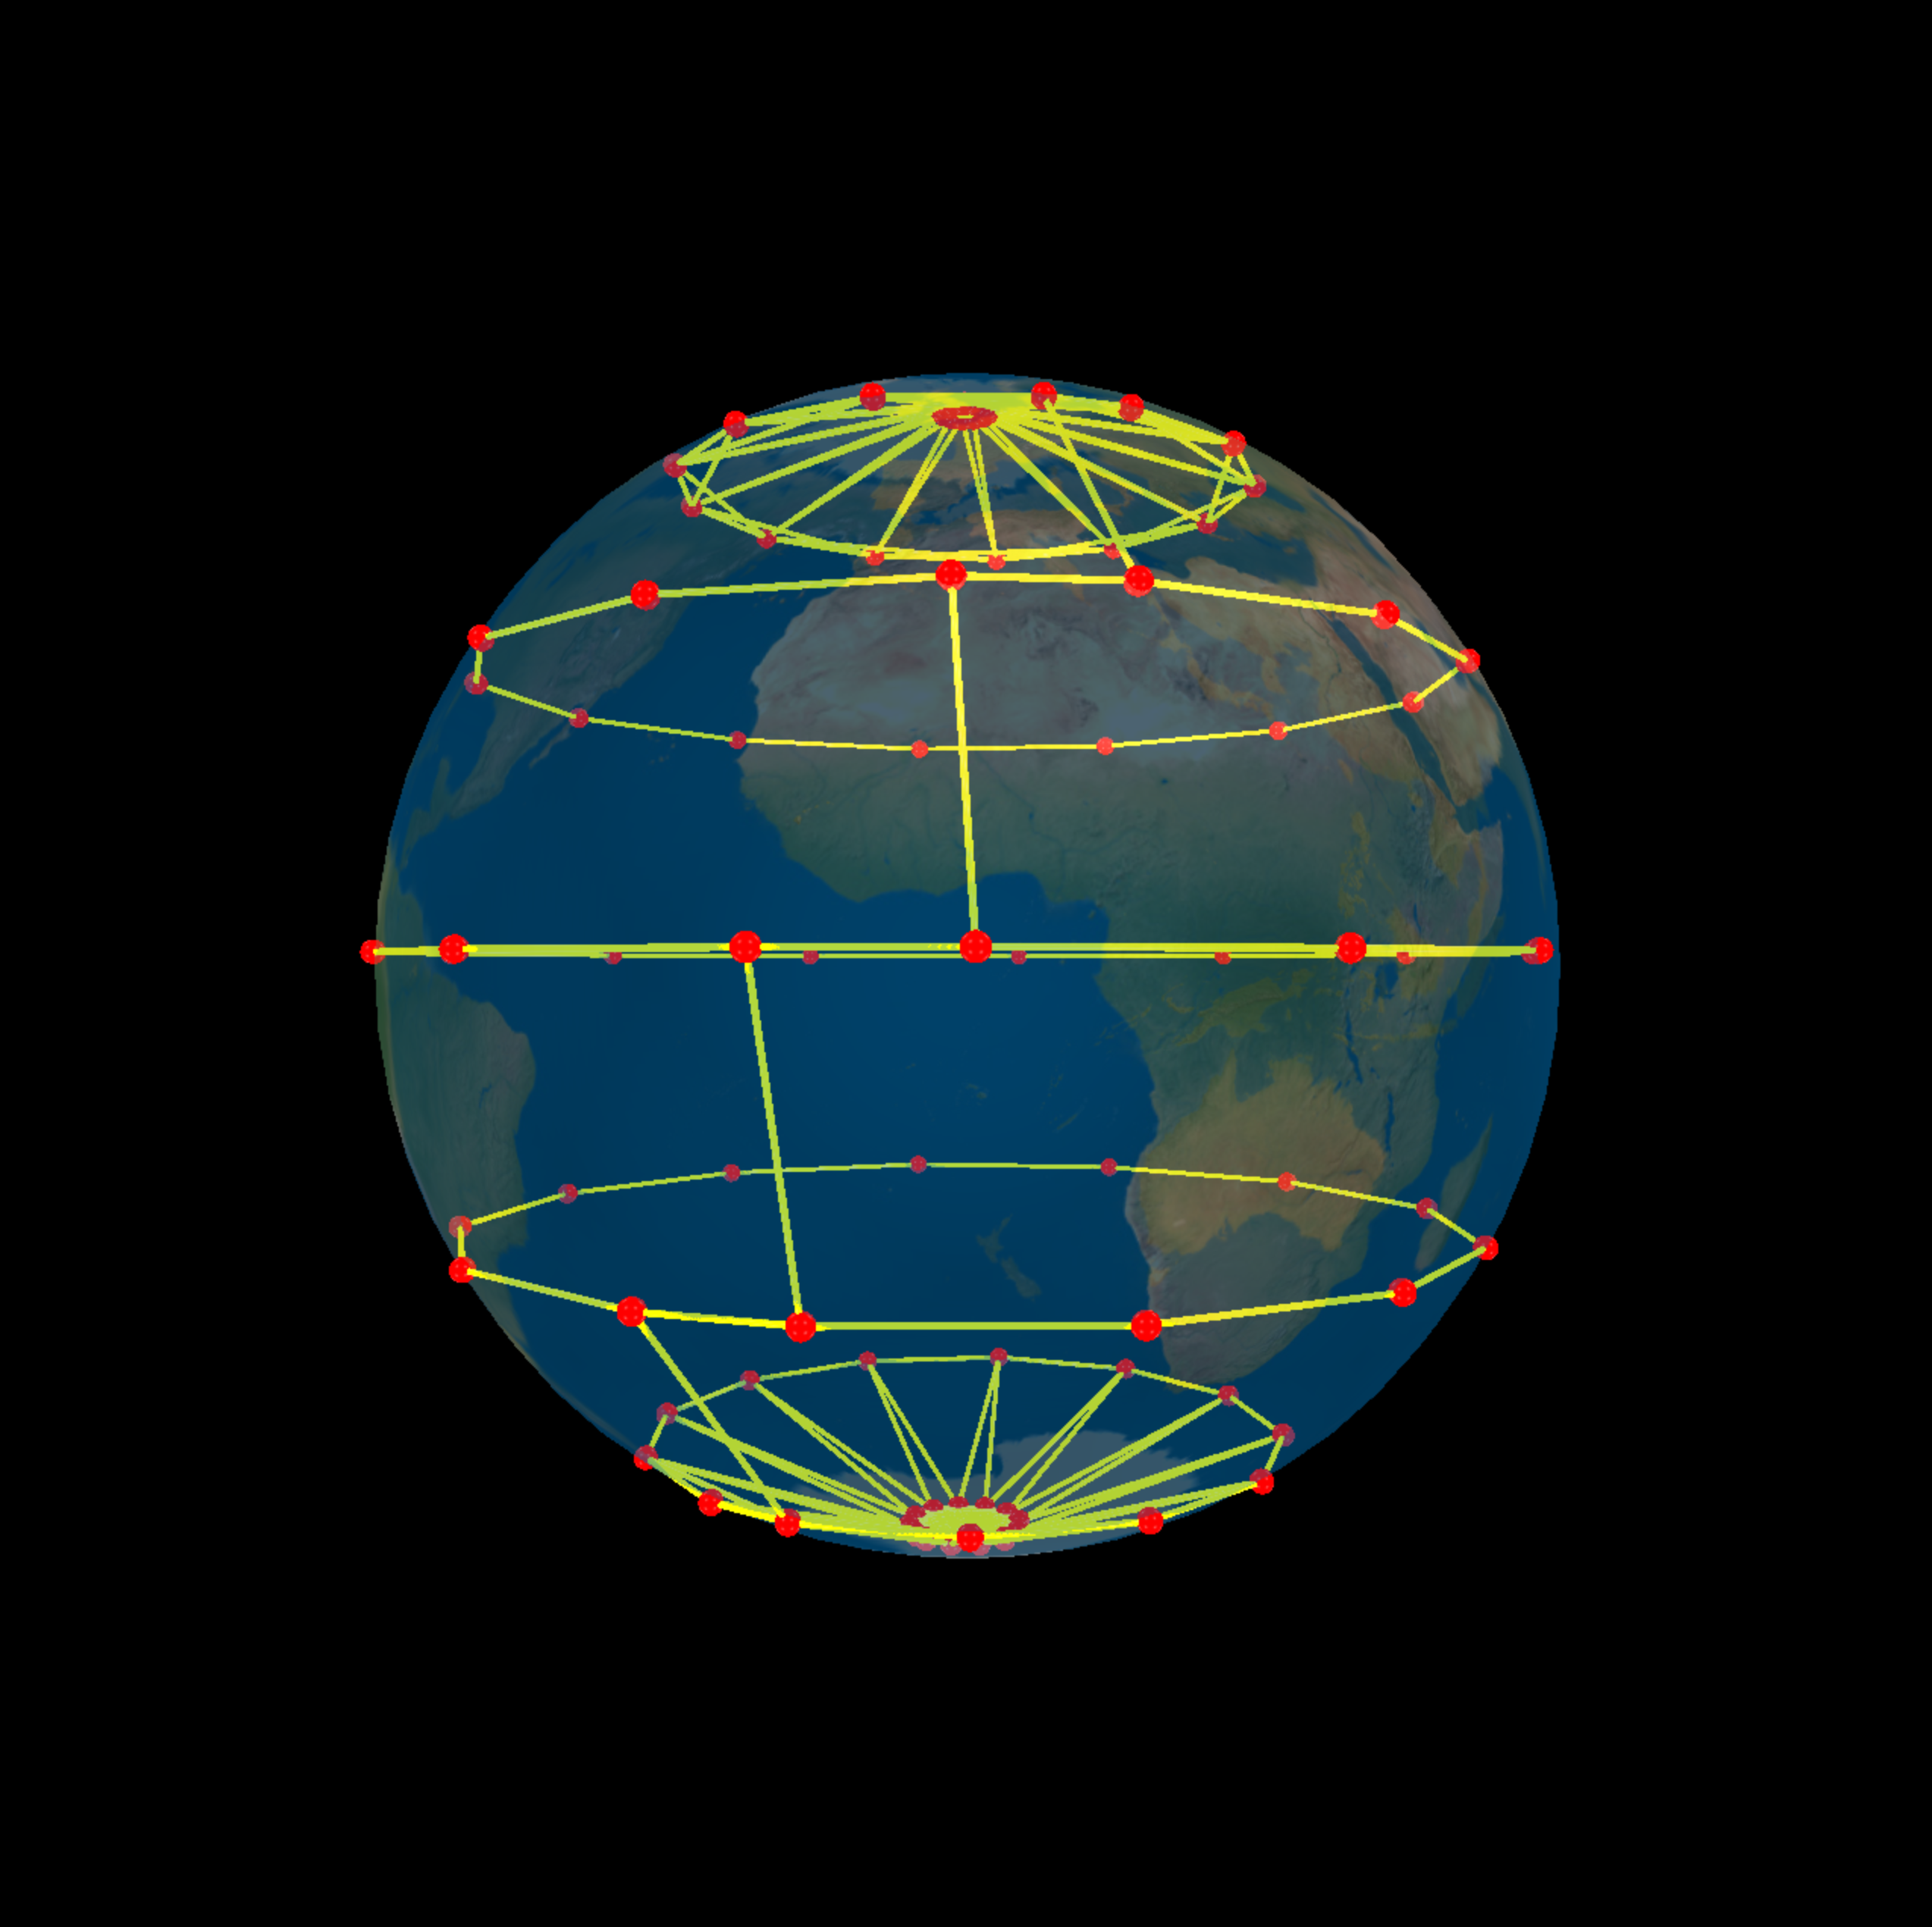
\includegraphics[scale=0.15]{used_images/connections02}
		\caption{Sensors 2: $r = 0.5$}
	\end{subfigure}%
	
\end{figure}
\end{frame}










\subsection{Čech complex $\longrightarrow$ $b_0 = 1 \wedge b_1 = 0$}

\begin{frame}{Čech complex $\longrightarrow$ $b_0 = 1 \wedge b_1 = 0$}
The sensor network should cover the whole sphere.
\begin{figure}[!ht]
	\centering
	\begin{subfigure}{.5\textwidth}
		\centering
		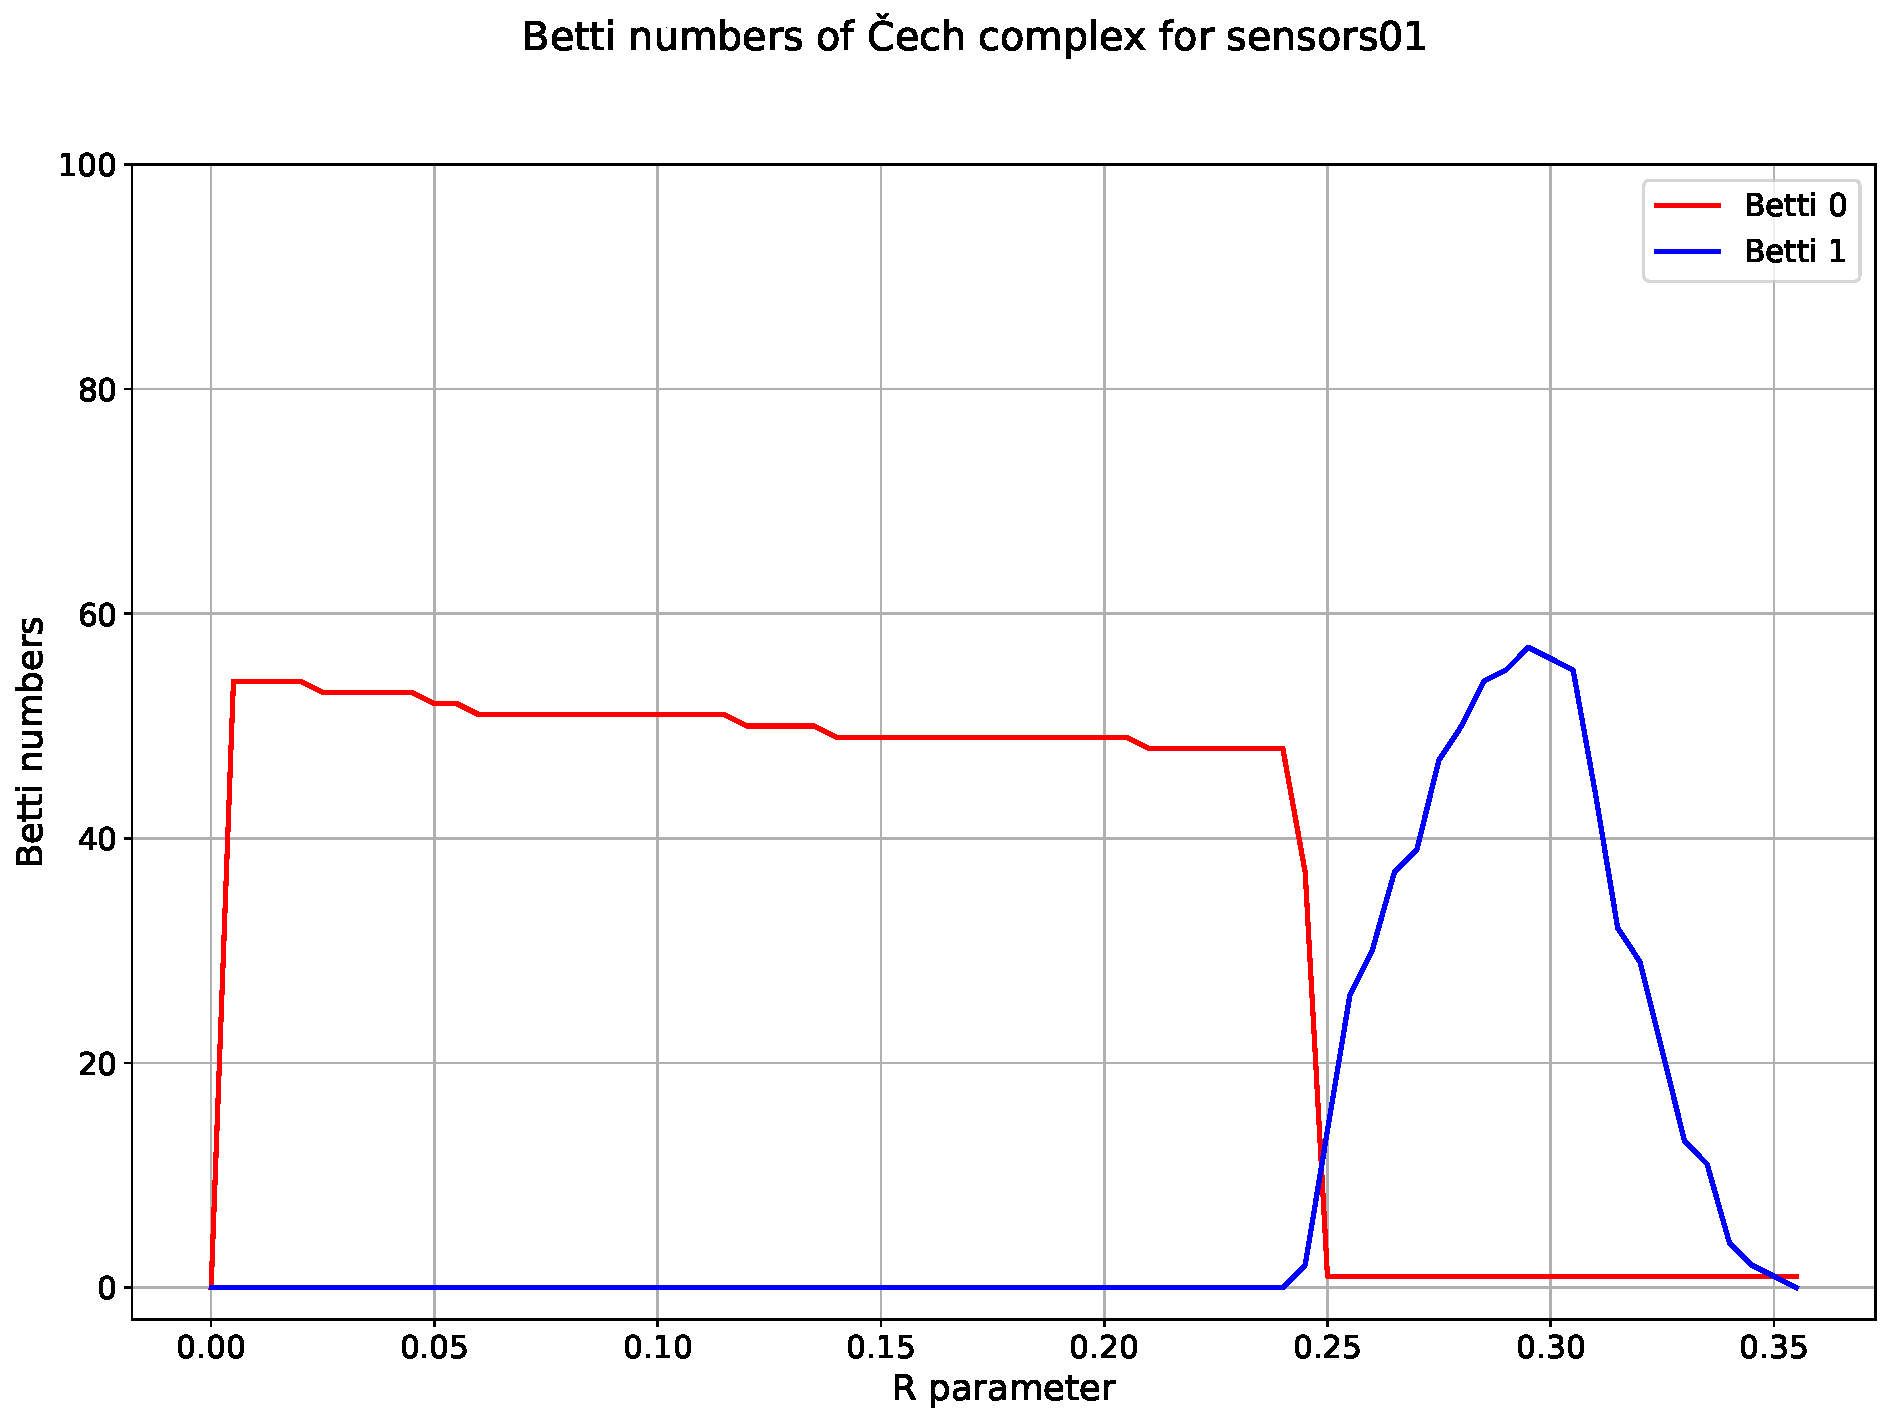
\includegraphics[scale=0.19]{used_images/plot_cech_sensors01.pdf}
		\caption{$R = 0.355$}
	\end{subfigure}%
	\begin{subfigure}{.5\textwidth}
		\centering
		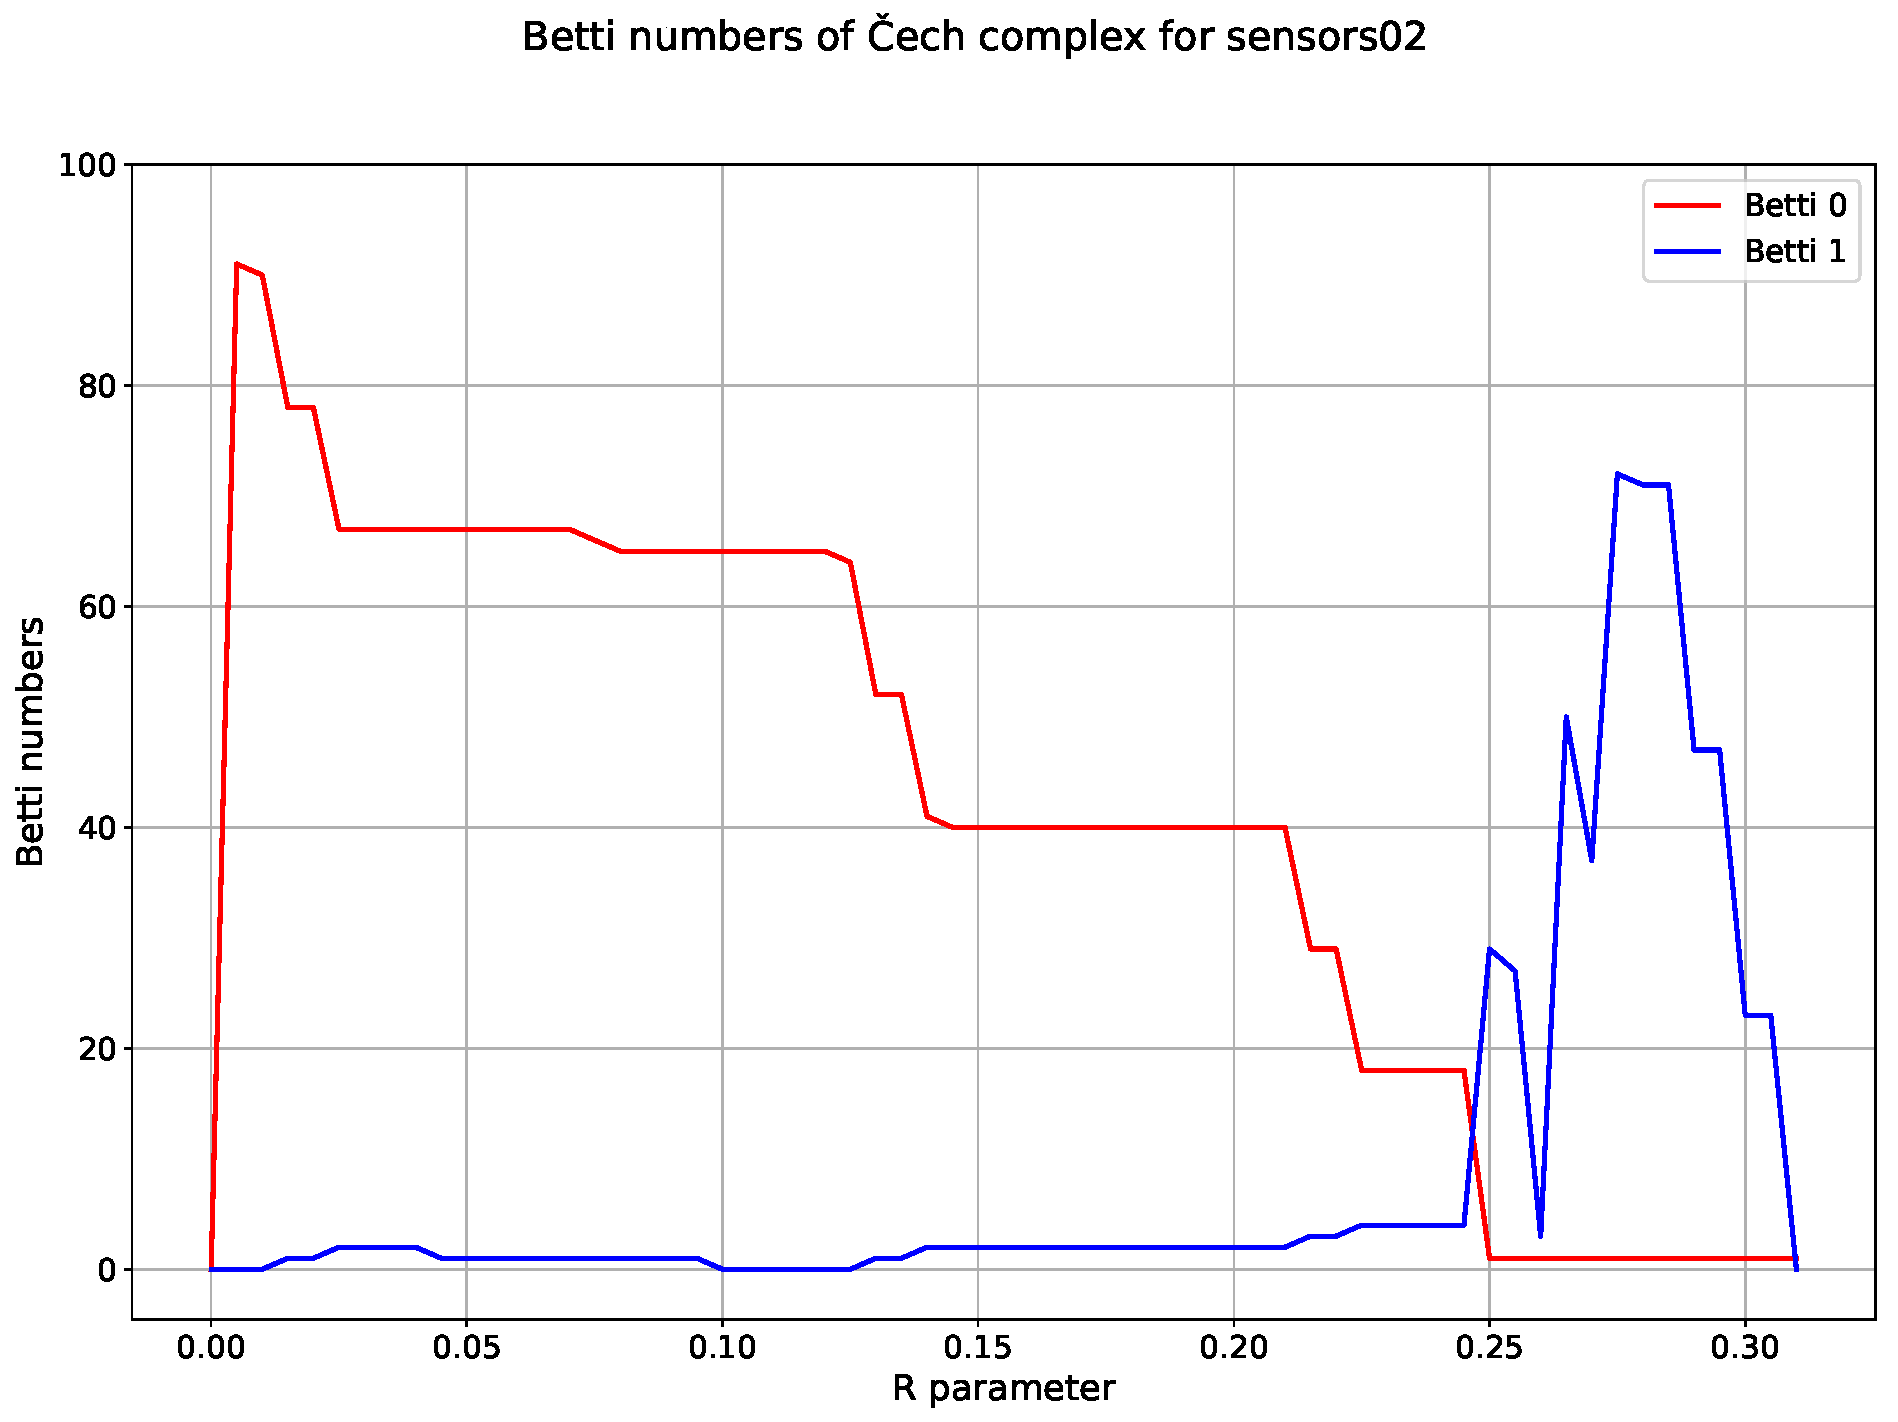
\includegraphics[scale=0.19]{used_images/plot_cech_sensors02.pdf}
		\caption{$R = 0.31$}
	\end{subfigure}%
	
\end{figure}
\end{frame}

\subsection{Barcode for Čech}

\begin{frame}{Barcode for Čech}

\begin{figure}[!ht]
\centering
\begin{subfigure}{.5\textwidth}
	\centering
	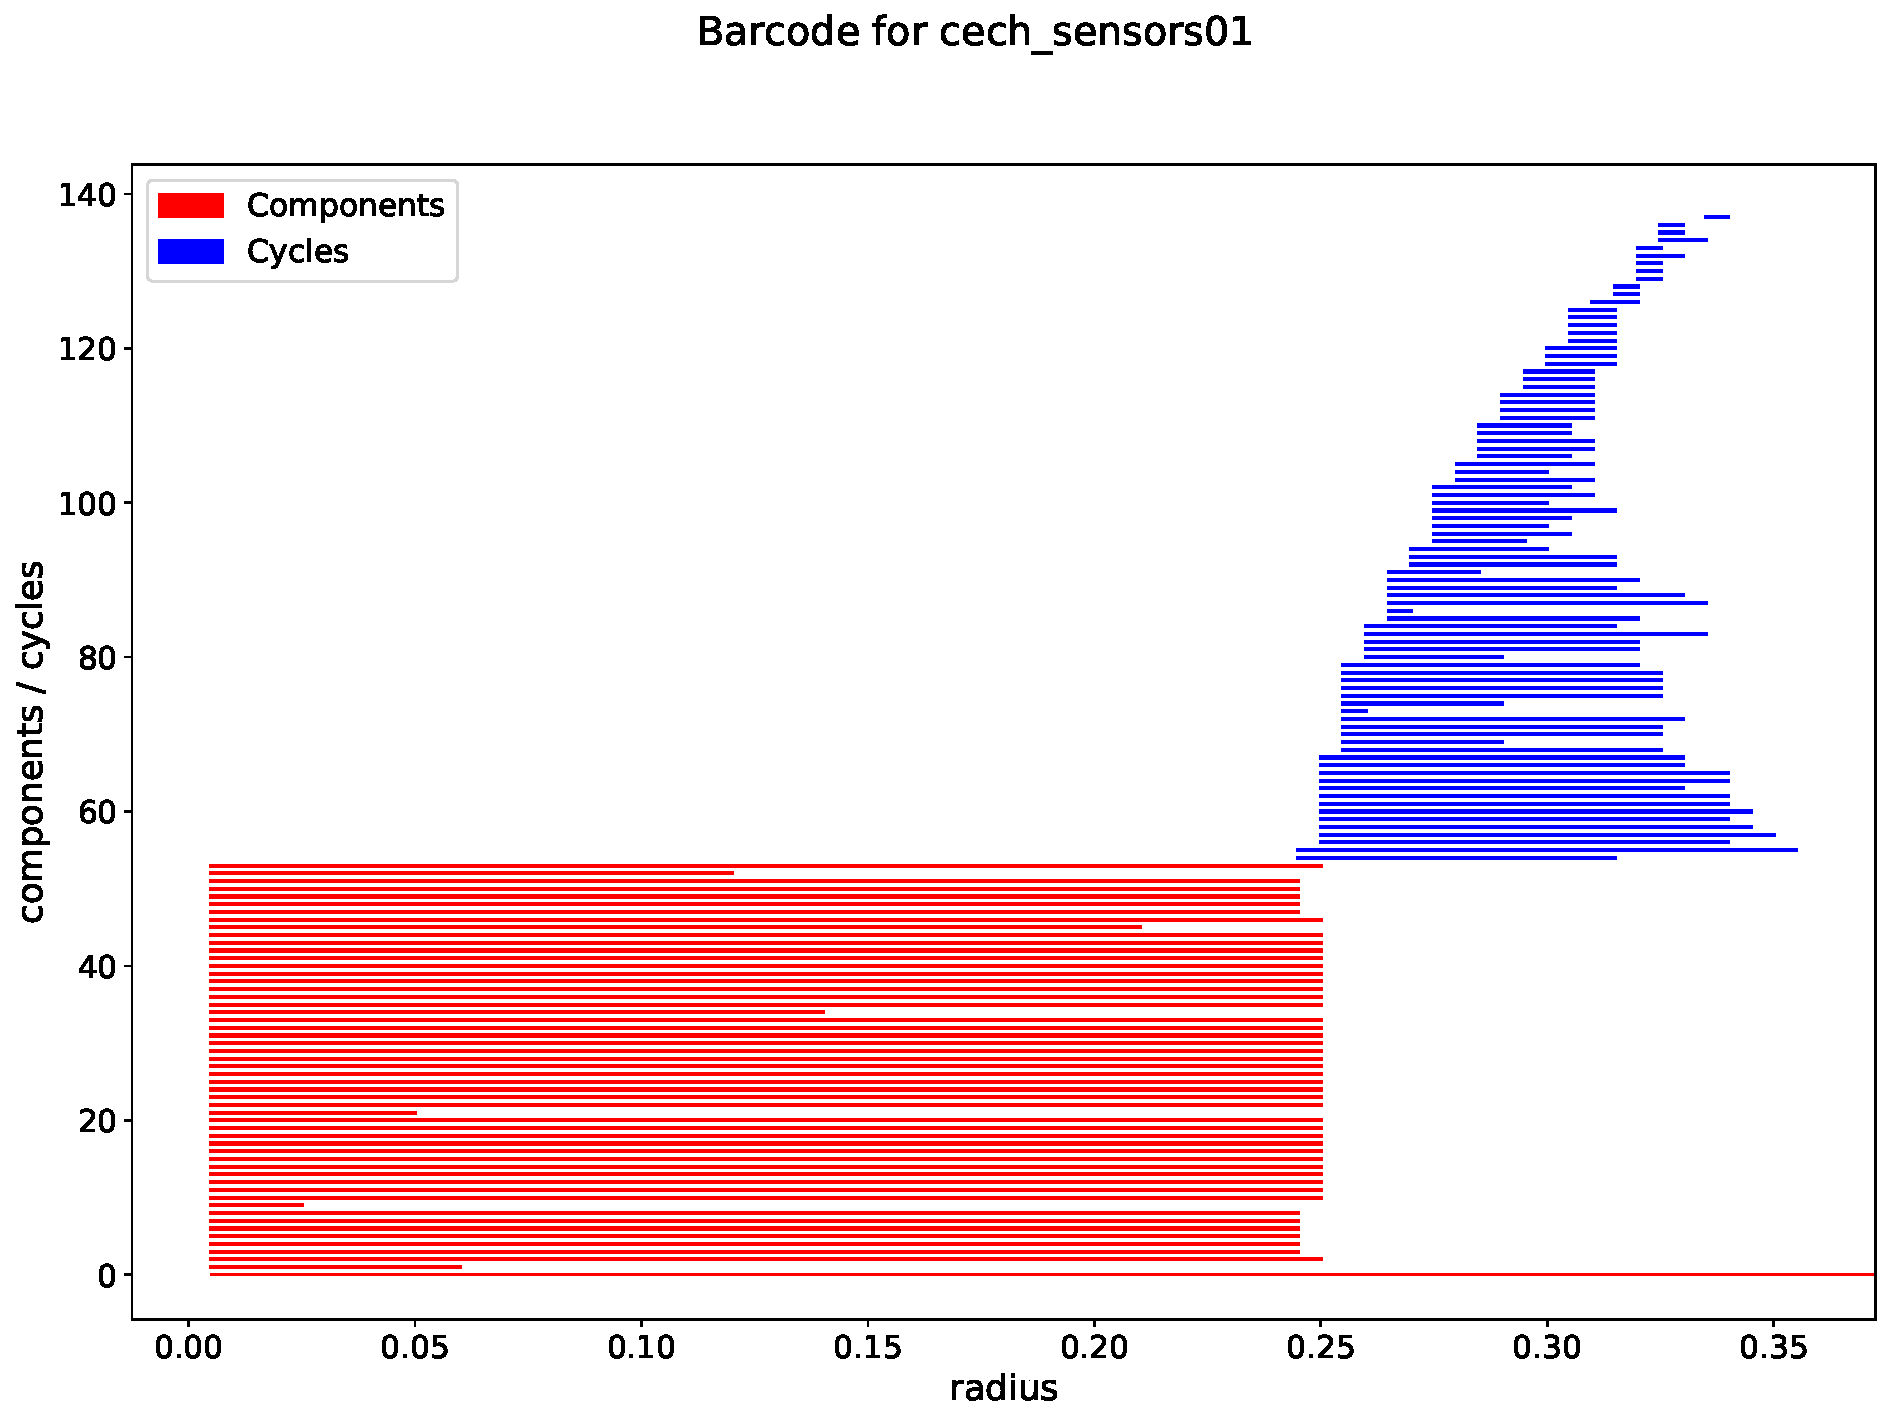
\includegraphics[scale=0.19]{used_images/barcode_cech_sensors01.pdf}
	\caption{Sensors 1.}
\end{subfigure}%
\begin{subfigure}{.5\textwidth}
	\centering
	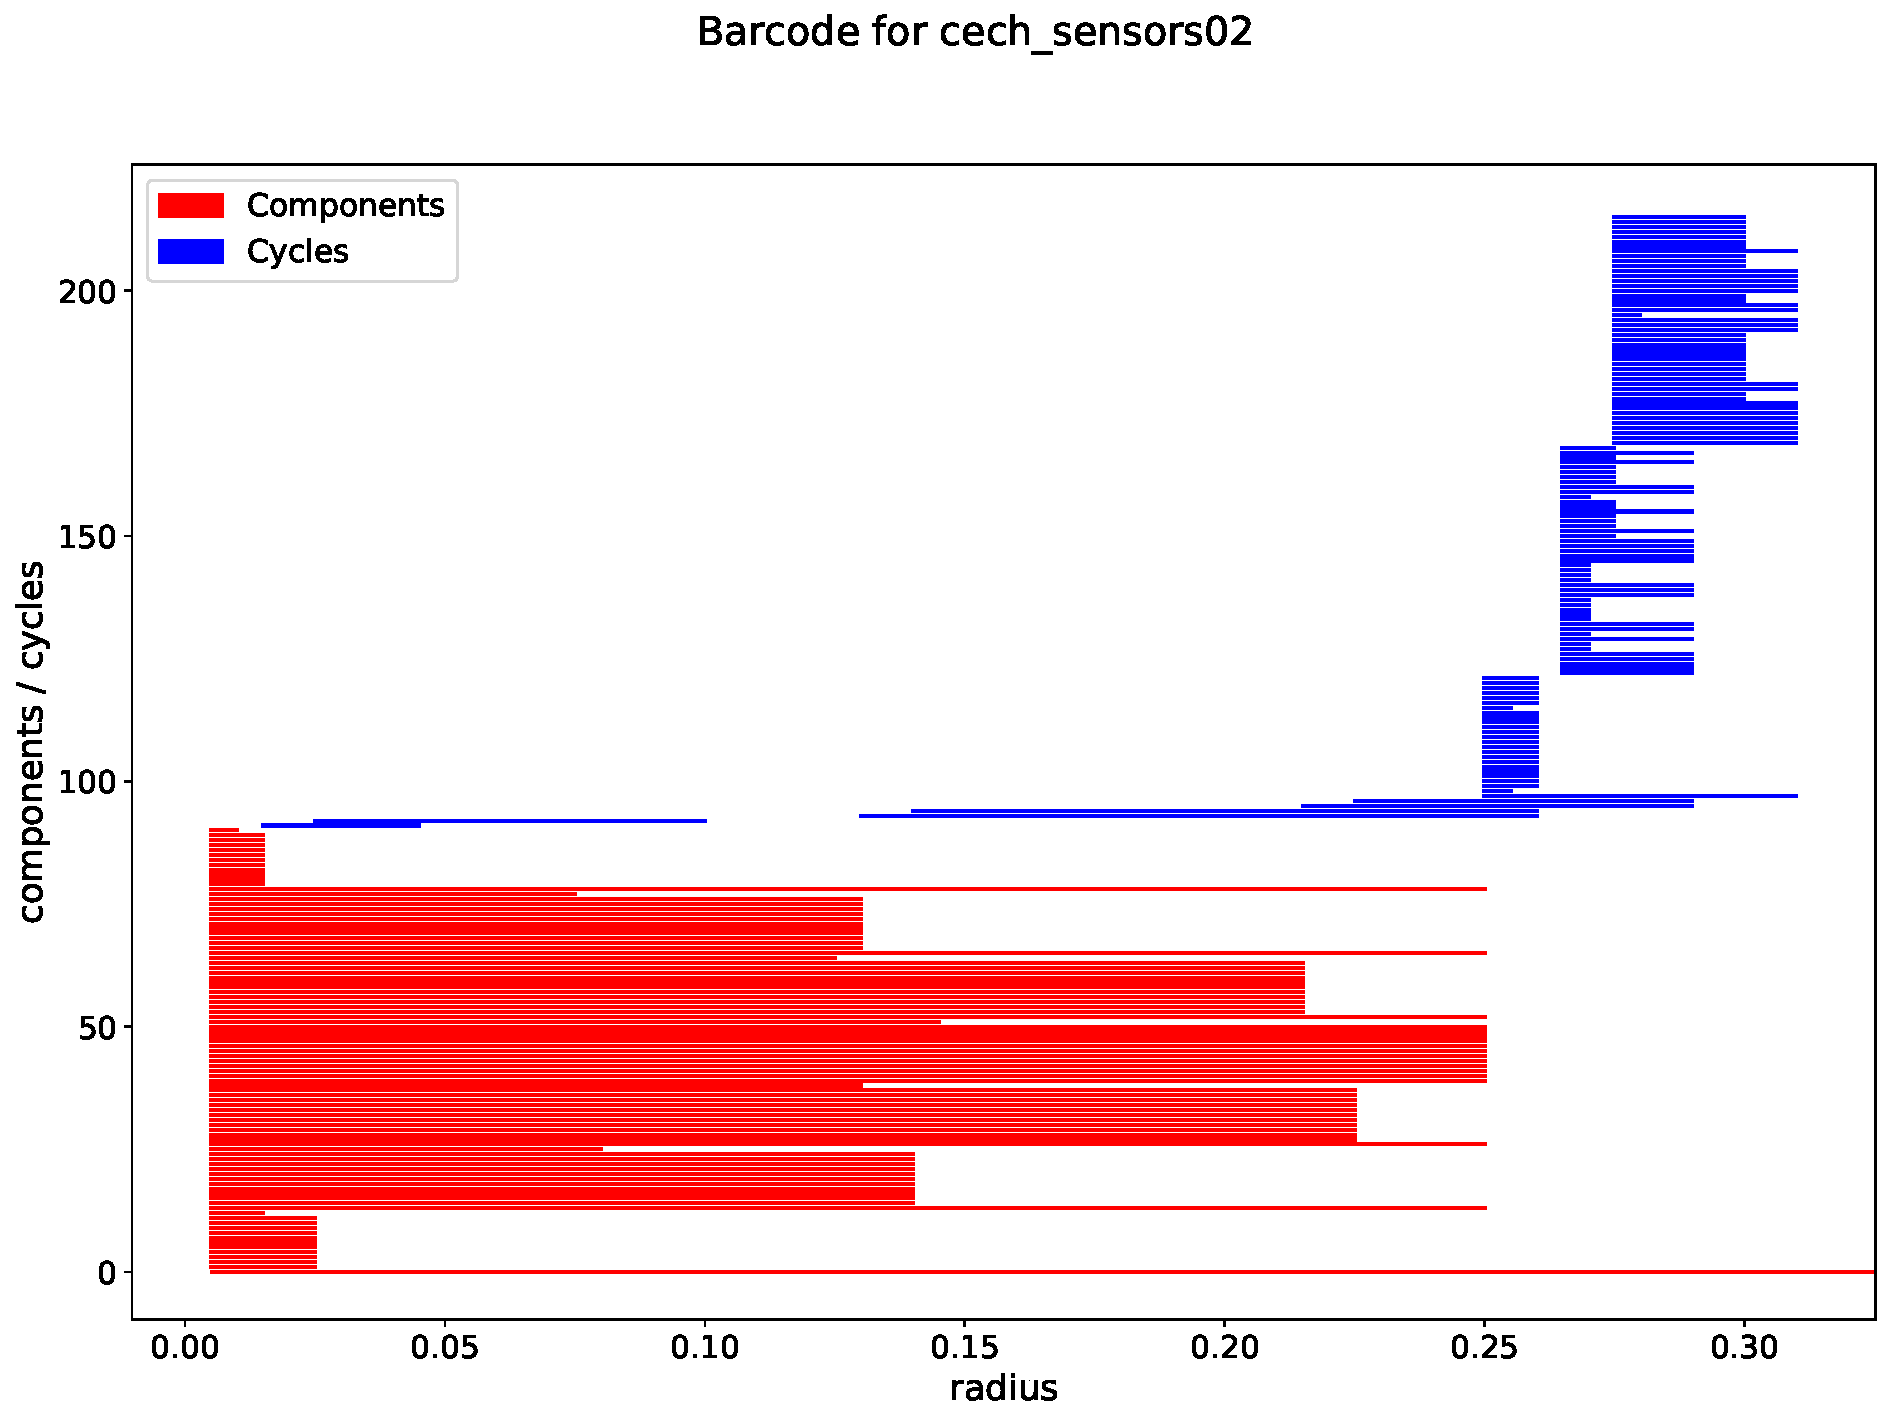
\includegraphics[scale=0.19]{used_images/barcode_cech_sensors02.pdf}
	\caption{Sensors 2.}
\end{subfigure}%

\end{figure}
\end{frame}
\subsection{Coverage in sensor network}
\begin{frame}{Coverage in sensor network}
Coverage in sensor network for appropriate parameter $R$.
\begin{figure}[!ht]
\centering
\begin{subfigure}{.5\textwidth}
\centering
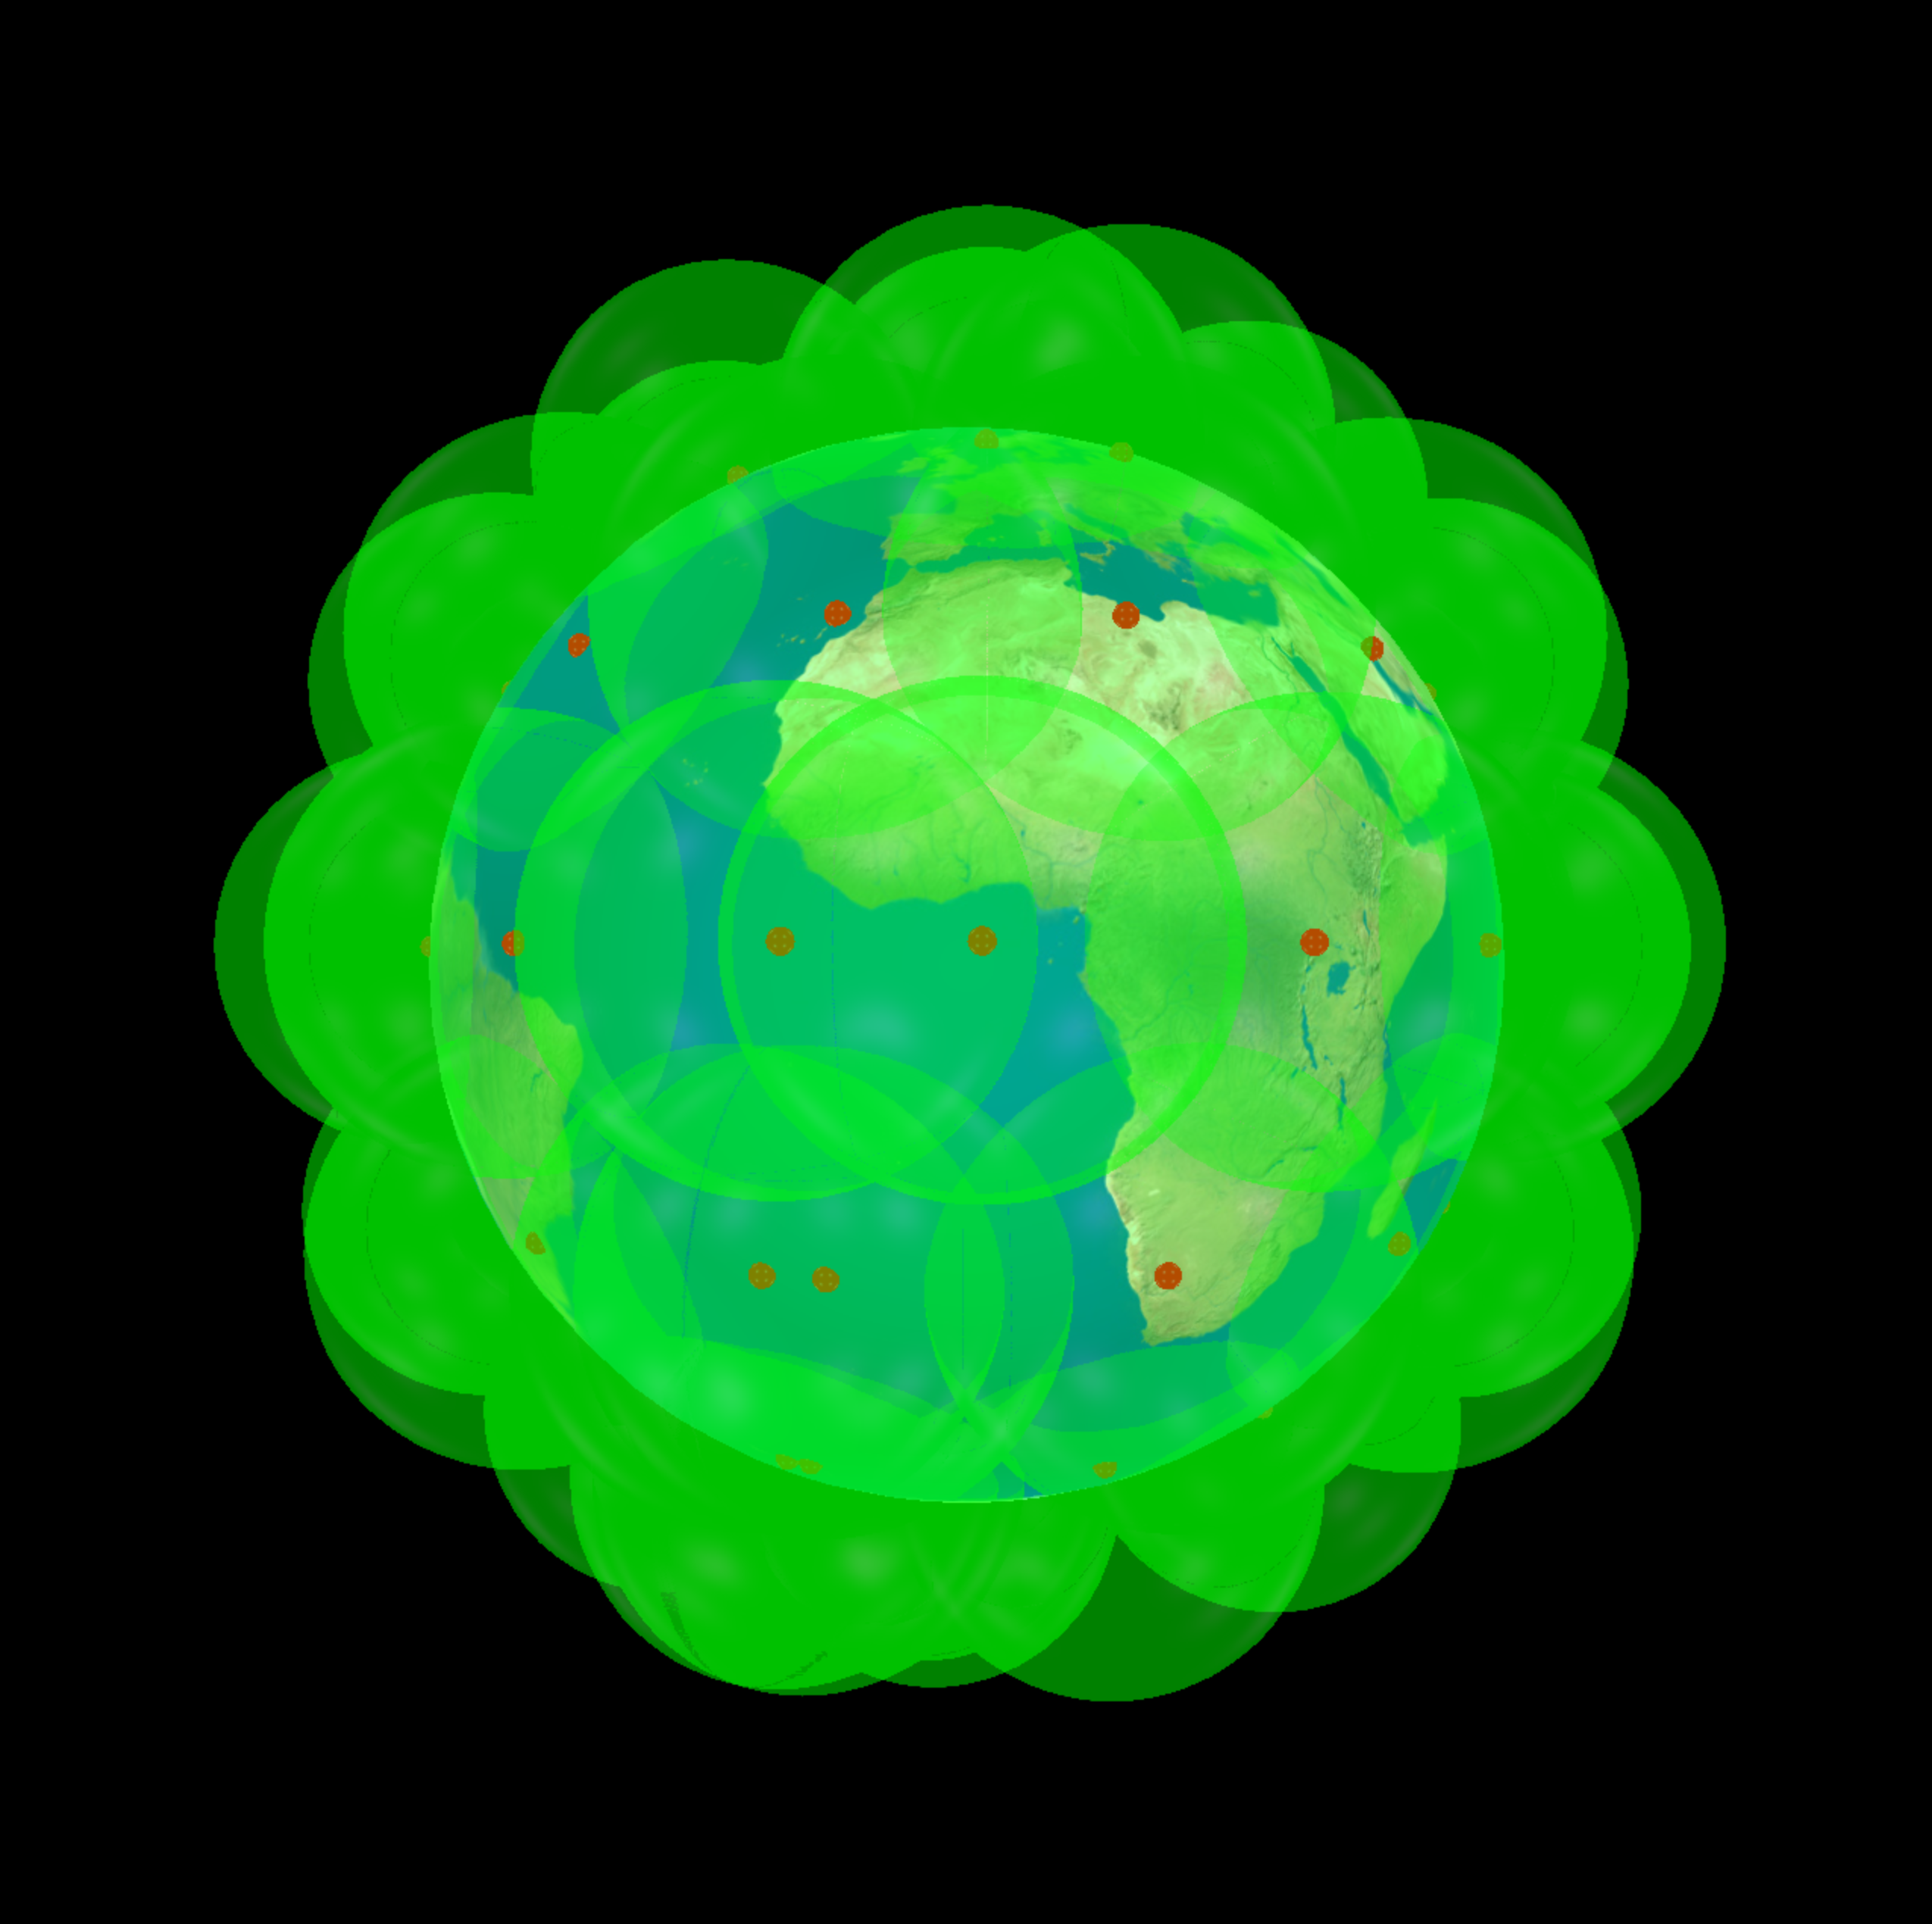
\includegraphics[scale=0.15]{used_images/coverage01}
\caption{Sensors 1: $R = 0.355$}
\end{subfigure}%
\begin{subfigure}{.5\textwidth}
\centering
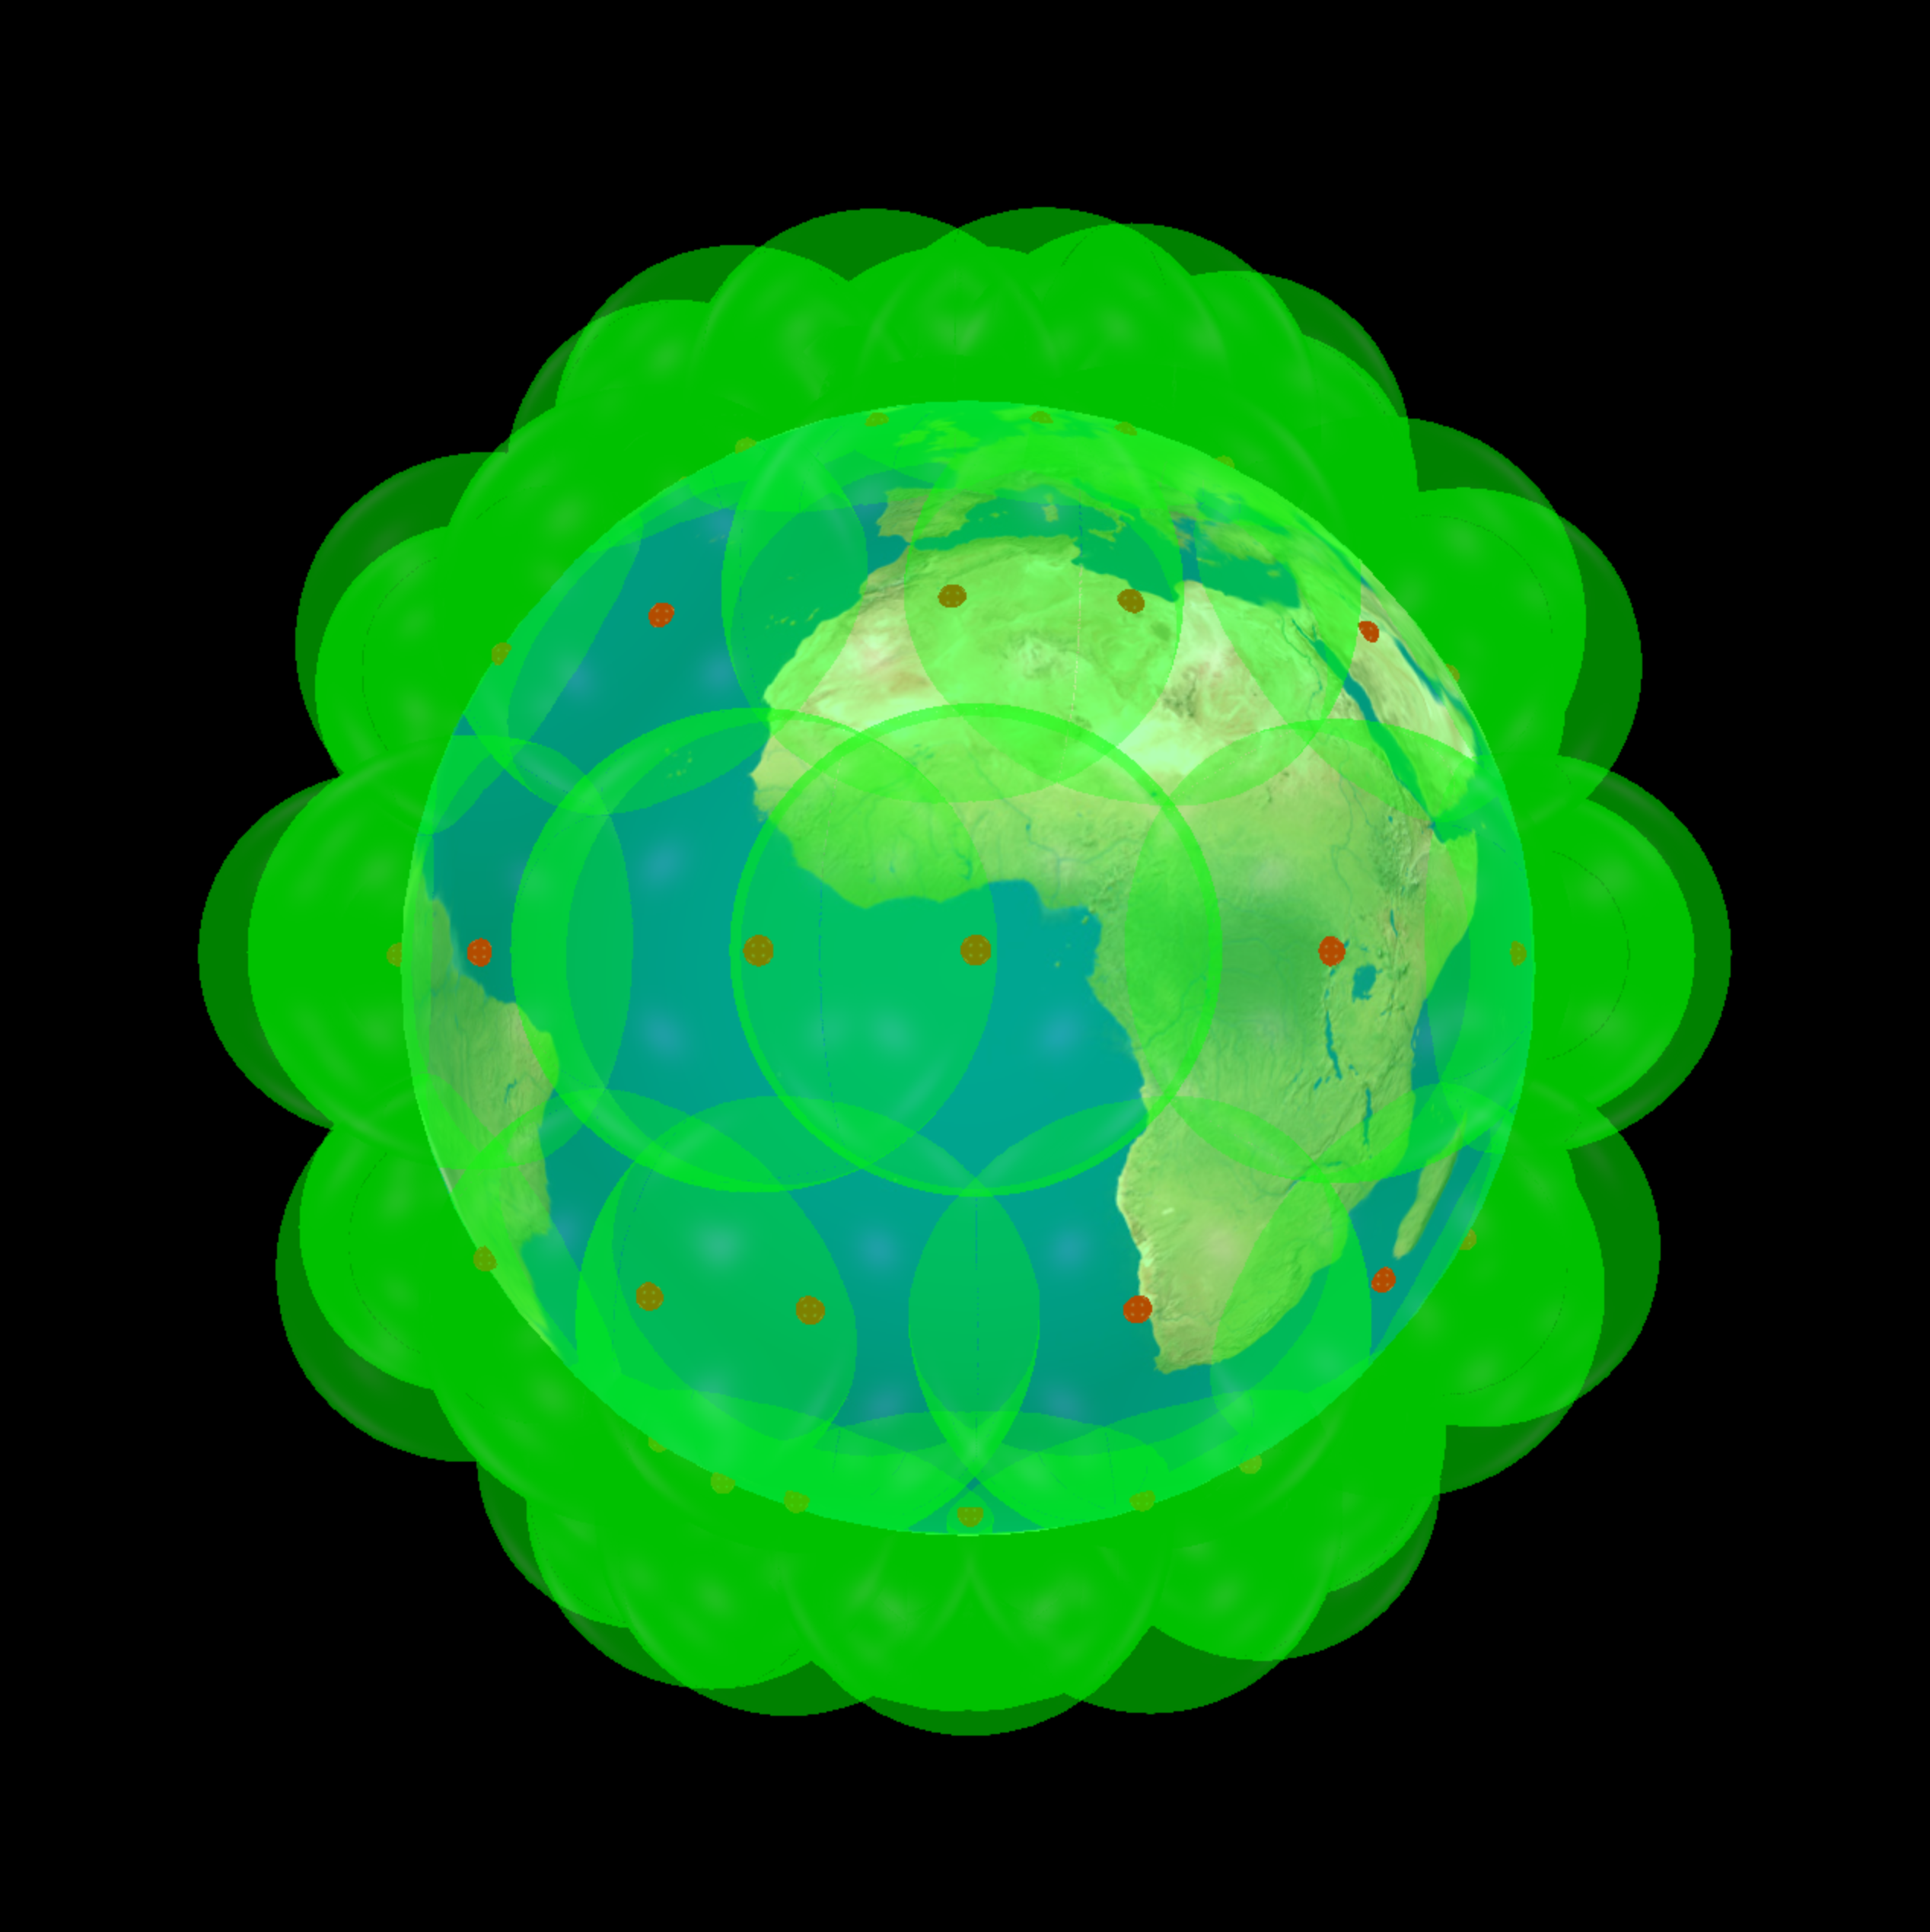
\includegraphics[scale=0.15]{used_images/coverage02}
\caption{Sensors 2: $R = 0.31$}
\end{subfigure}%

\end{figure}
\end{frame}


\subsection{Redundant sensors}
\begin{frame}{Redundant sensors}{}
We looked for redundant sensors with a simple algorithm:
\begin{itemize}
	\item ignore cut vertices of the VR complex (they separate the network in multiple components),
	\item ignore points with less than 3 neighbors in radius $R$ (they create holes in Čech complex),
	\item randomly select points from the remaining list and check if removing them would break our solution
	\item optionally, check all ways of removing any vertices from the remaining list, if it is small enough (exhaustive search)
\end{itemize}
In this way we got a compromise between finding the best solution and spent time

\end{frame}





\subsection{Data generator}
\begin{frame}{Data generator}{}
Distribution of points on the sphere so that parameters $r$ and $R$ are as small as possible.
\begin{alertblock}{Coulomb's law}
	\centering $|\vect{F_{ij}}| = k_e \frac{e^2}{|\vect{r_i}-\vect{r_j}|^2}$
\end{alertblock}
\begin{alertblock}{Electrostatic potential energy}
	\centering $V = \sum_{i\neq j}V_{ij} \propto \sum_{i\neq j}\frac{1}{|\vect{r_i} - \vect{r_j}|}$
\end{alertblock}
\begin{itemize}
	\item {Electrons would distribute themselves evenly around the sphere. }
	\item {Minimization of $V$ with simulated annealing.}
\end{itemize}

\end{frame}

\subsection{Algorithm for MC simulated annealing}
\begin{frame}{Algorithm for MC simulated annealing}
\begin{enumerate}
	\item {Start with random distribution of points on sphere.}
	\item {Set initial temperature of the system $T$.}
	\item {Choose random point, move it according to Gaussian distribution.}
	\item {Calculate difference in energy $\Delta E$.}
	\item {If $\Delta E < 0$, accept the change.} 
	\item {If $\Delta E \geq 0$, accept the change with probability $\exp(\frac{-\Delta E}{T})$}
	\item {If enough changes accepted, decrease the temperature $T$.}
	\item {Repeat process from 3. $\longrightarrow$}
\end{enumerate}
\end{frame}

\begin{frame}{Results for $n=4$ and $n=50$}
\begin{figure}[!ht]
	\centering
	\begin{subfigure}{.5\textwidth}
		\centering
		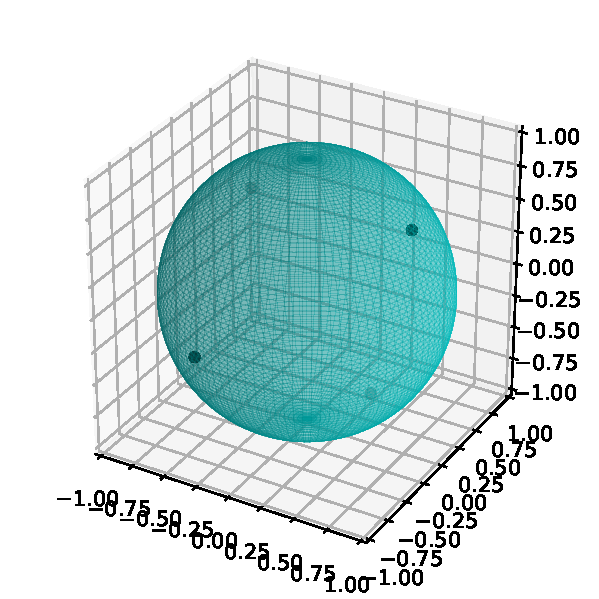
\includegraphics[scale=0.6]{used_images/generated2.pdf}
		\caption{n = 4}
	\end{subfigure}%
	\begin{subfigure}{.5\textwidth}
		\centering
		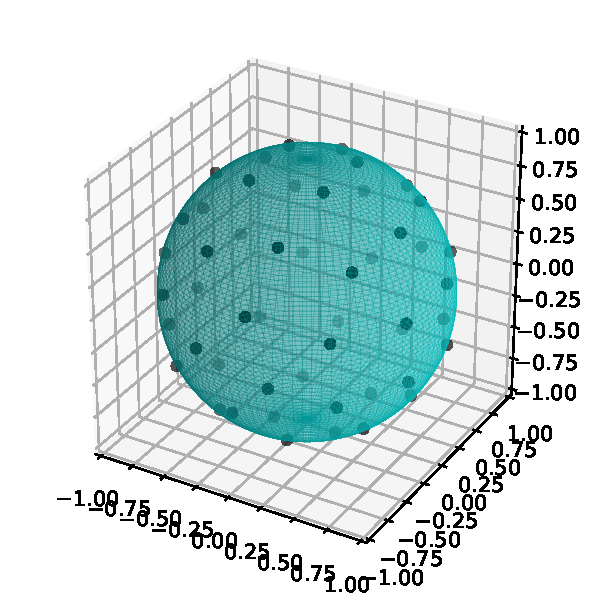
\includegraphics[scale=0.6]{used_images/generated1.pdf}
		\caption{n = 50}
	\end{subfigure}%

\end{figure}
\end{frame}

\section*{Summary}

\begin{frame}{Summary}
Thank you for listening. 
\end{frame}





\begin{frame}
  \frametitle<presentation>{Bibliography}
    
  \begin{thebibliography}{99}

  \setbeamertemplate{bibliography item}[online]
  	 
  \bibitem{A}Vietoris-Rips. \url{https://en.wikipedia.org/wiki/Vietoris_Rips_complex} (5.6.2018).
  \bibitem{A}Čech-complex. \url{https://en.wikipedia.org/wiki/Cech_complex} (5.6.2018).
  \setbeamertemplate{bibliography item}[book]
 	
  \bibitem{B} Lecture notes from prof. dr. Neža Mramor Kosta.
  \end{thebibliography}
\end{frame}

\end{document}


